\chapter{Đánh giá thực nghiệm và Kết quả}
\label{ch:evaluation}

Chương này trình bày toàn diện phương pháp luận kiểm thử, quy trình thực nghiệm và các kết quả định lượng đạt được của nền tảng VietForecast dựa trên các nguyên tắc thiết kế và giải pháp hiện thực đã được đề xuất tại Chương~\ref{ch:architecture} và Chương~\ref{ch:implementation}. Mục tiêu trọng tâm của quá trình thực nghiệm nhằm kiểm chứng năm luận điểm kỹ thuật cốt lõi: (1) hiệu quả của giải thuật định tuyến Weather-Safer trong việc giảm thiểu phơi nhiễm trước các hiểm họa thời tiết cực đoan trên ba hành lang giao thông huyết mạch quốc gia; (2) khả năng phân hóa rủi ro đa chiều theo phương tiện di chuyển (ô tô con và xe máy hai bánh); (3) hiệu năng và độ trễ xử lý của cơ chế truy vấn không gian hai giai đoạn trên hệ cơ sở dữ liệu PostGIS kết hợp tầng nhớ đệm Redis; (4) độ chính xác kích hoạt công cụ nghiệp vụ, tính kiểm chứng dữ liệu thực địa và khả năng tự phục hồi của trợ lý AI đàm thoại; và (5) mức độ tiện dụng, tính trực quan và sự hài lòng của người dùng khi tương tác với giao diện bản đồ số thông qua thang đo chuẩn mực quốc tế SUS (\textit{System Usability Scale}).

\section{Thiết lập Môi trường Thực nghiệm và Kịch bản Kiểm thử Hành lang}
\label{sec:experimental_setup}

\subsection{Cấu hình Hạ tầng Phần cứng và Phần mềm Thử nghiệm}
Quá trình đo kiểm thực nghiệm được triển khai trên môi trường máy chủ phân tán đồng nhất nhằm bảo đảm tính lặp lại và độ tin cậy khoa học của các số liệu đo lường:
\begin{itemize}
    \item[-] \textit{Hạ tầng phần cứng máy chủ}: Vi xử lý 8 nhân / 16 luồng xung nhịp cơ sở 3,20~GHz, bộ nhớ trong 32~GB RAM DDR4 ECC, ổ cứng thể rắn thể rắn NVMe PCIe 4.0 dung lượng 500~GB với băng thông đọc ghi ngẫu nhiên đạt trên 450.000~IOPS, và kết nối mạng nội bộ 1~Gbps song công toàn phần (\textit{full-duplex}).
    \item[-] \textit{Môi trường phần mềm và dịch vụ}: Hệ điều hành Ubuntu Server 24.04 LTS x86\_64 (nhân Linux 6.8.0), nền tảng ảo hóa Docker Engine 26.1 và Docker Compose v2.27. Cơ sở dữ liệu không gian PostgreSQL 16.3 đi kèm phần mở rộng PostGIS 3.4.2; hệ thống lưu trữ khóa--giá trị trong bộ nhớ Redis 7.2.4 Alpine; máy chủ ứng dụng Node.js v20.14 LTS chạy Fastify 5.0 và TypeScript 5.5.
    \item[-] \textit{Công cụ sinh tải và đo lường}: Công cụ kiểm thử hiệu năng k6 v0.51 và Autocannon v7.15 được sử dụng để giả lập tải đồng thời từ 50 đến 1.000 người dùng ảo (\textit{Virtual Users -- VUs}) với các kịch bản truy vấn ngẫu nhiên và truy vấn dồn dập (\textit{spike testing}).
\end{itemize}

\subsection{Ba Hành lang Giao thông Trọng điểm Quốc gia}
Để đánh giá toàn diện tính thực tiễn của hệ thống trong điều kiện khí hậu nhiệt đới gió mùa đa dạng của Việt Nam, ba hành lang giao thông huyết mạch với đặc tính địa lý và hình thế thời tiết hoàn toàn khác biệt đã được lựa chọn làm tập mẫu thực nghiệm:
\begin{itemize}
    \item[-] \textit{Hành lang Vùng núi Phía Bắc (Hà Nội -- Lào Cai / Sa Pa)}: Tuyến có tổng cự ly từ 287~km đến 315~km kết nối trung tâm đồng bằng Bắc Bộ với vùng cao biên giới Tây Bắc. Đặc thù địa hình chuyển tiếp đột ngột từ cao độ 15~m lên trên 1.500~m so với mực nước biển, đường sá có độ dốc lớn và nhiều khúc cua tay áo. Rủi ro khí tượng chủ đạo gồm sương mù dày đặc che khuất tầm nhìn, mưa dông đối lưu cục bộ cường suất cao gây nguy cơ sạt lở taluy dương và trơn trượt lòng đường.
    \item[-] \textit{Hành lang Duyên hải Miền Trung (Đà Nẵng -- Thừa Thiên Huế)}: Tuyến có cự ly khoảng 100~km kết nối hai đô thị trọng điểm qua dãy Bạch Mã, bao gồm hai phương án tuyến: vượt đèo Hải Vân (đường đèo hiểm trở sát biển) hoặc đi xuyên hầm đường bộ Hải Vân. Rủi ro khí tượng đặc thù gồm gió tạt ngang cực mạnh trên đỉnh đèo và các cầu cạn vượt biển (gió giật cấp 7--8), mưa lớn dồn dập trong mùa bão gây hiện tượng thủy phi cơ (\textit{aquaplaning}) nguy hiểm cho phương tiện chạy tốc độ cao.
    \item[-] \textit{Hành lang Xuyên Việt Bắc -- Nam (Hà Nội -- TP. Hồ Chí Minh)}: Trục giao thông huyết mạch dài 1.720~km trải dài dọc theo Quốc lộ 1A và các đoạn đường bộ cao tốc Bắc -- Nam. Tuyến di chuyển cắt ngang qua bốn miền khí hậu khác nhau (Bắc Bộ, Bắc Trung Bộ, Duyên hải Nam Trung Bộ và Nam Bộ), đòi hỏi thuật toán định tuyến phải liên tục dự phóng và bù trừ thời gian di chuyển ước tính (ETA) để đánh giá sự giao thoa giữa phương tiện và các tâm bão di động theo thời gian thực.
\end{itemize}

\subsection{Kịch bản Kiểm thử Khí tượng Cực đoan và Tiêu chí Định lượng}
Để kiểm thử giới hạn chịu đựng và tính nhạy cảm của thuật toán, hệ thống kết hợp dữ liệu quan trắc thời gian thực tế từ mạng lưới trạm tự động với phương pháp tiêm nhiễu thời tiết cực đoan nhân tạo (\textit{synthetic weather injection}):
\begin{itemize}
    \item[-] \textit{Ngưỡng mưa dông cực đoan}: Cường độ mưa tức thời vượt mức 25~mm/h đến 50~mm/h kèm hoạt động dông sét đối lưu mạnh.
    \item[-] \textit{Ngưỡng gió tạt nguy hiểm}: Tốc độ gió duy trì trên 40~km/h hoặc gió giật tức thời vượt mức 55~km/h (tương đương gió cấp 7 trở lên trên thang sức gió Beaufort).
    \item[-] \textit{Ngưỡng tầm nhìn suy giảm}: Tầm nhìn xa khí quyển giảm xuống dưới 500~m do sương mù bức xạ hoặc mưa rào cường độ mạnh.
\end{itemize}

Các chỉ số đánh giá định lượng được chuẩn hóa bao gồm: Điểm rủi ro lộ trình tích lũy $R_{\text{route}} \in [0, 1]$, Tỷ lệ checkpoint thời tiết nguy hiểm bị loại bỏ ($\Delta\text{Hazard}$), Mức tăng thời gian di chuyển ($\Delta T_{\text{travel}}$), và Mức tăng khoảng cách địa lý ($\Delta D_{\text{distance}}$).

\section{Đánh giá Hiệu quả Thuật toán Giảm thiểu Rủi ro Tuyến đường}
\label{sec:route_risk_mitigation}

\subsection{So sánh Định lượng Đa Phương án Lộ trình}
Hệ thống tính toán và so sánh song song ba phương án di chuyển độc lập cho mỗi yêu cầu định tuyến:
\begin{itemize}
    \item[-] \textit{Phương án Nhanh nhất (Fastest)}: Tối ưu hóa tuyệt đối theo thời gian lưu thông trên trục đường cao tốc tiêu chuẩn, không né tránh các vùng rủi ro thời tiết.
    \item[-] \textit{Phương án Ngắn nhất (Shortest)}: Tối ưu hóa theo quãng đường di chuyển ngắn nhất trên bản đồ mạng lưới giao thông đường bộ.
    \item[-] \textit{Phương án An toàn Thời tiết nhất (Weather-Safer)}: Điều chỉnh hàm mục tiêu chi phí bằng cách gán trọng số phạt rủi ro khí quyển, chủ động điều hướng phương tiện vòng qua các vùng thời tiết nguy hiểm hoặc khuyến nghị hạ tốc độ tại các điểm trọng yếu.
\end{itemize}

Bảng~\ref{tab:corridor_eval_vi} tổng hợp kết quả thực nghiệm chi tiết trên ba hành lang giao thông kiểm thử dưới điều kiện hình thái thời tiết có bão và mưa dông đối lưu.

\begin{table}[htbp]
\centering
\caption[So sánh hiệu quả định lượng giữa các phương án di chuyển]{So sánh hiệu quả định lượng giữa ba phương án di chuyển trên ba hành lang giao thông kiểm thử trọng điểm.}
\label{tab:corridor_eval_vi}
\begin{adjustbox}{width=\textwidth,center}
\begin{tabular}{llcccccc}
\toprule
\textbf{Hành lang kiểm thử} & \textbf{Phương án lộ trình} & \textbf{Cự ly (km)} & \textbf{Thời gian} & \textbf{Điểm rủi ro ($R$)} & \textbf{Cấp rủi ro} & \textbf{Điểm nguy hiểm} & \textbf{Mức tăng $\Delta T$} \\
\midrule
\multirow{3}{*}{\shortstack[l]{Hà Nội -- Lào Cai\\(Cự ly chuẩn $\sim 287$~km)}} 
  & Nhanh nhất (Cao tốc) & 287 & 3h 54m & 0,68 & Nguy hiểm (Đỏ) & 4 / 6 & -- \\
  & Ngắn nhất (QL70) & 275 & 5h 30m & 0,42 & Chú ý (Vàng) & 2 / 6 & +41,0\% \\
  & \textbf{Weather-Safer (Đề xuất)} & \textbf{298} & \textbf{4h 20m} & \textbf{0,14} & \textbf{An toàn (Xanh)} & \textbf{0 / 6} & \textbf{+11,1\%} \\
\midrule
\multirow{3}{*}{\shortstack[l]{Đà Nẵng -- Huế\\(Cự ly chuẩn $\sim 100$~km)}} 
  & Nhanh nhất (Đèo Hải Vân) & 96 & 2h 15m & 0,74 & Nguy hiểm (Đỏ) & 3 / 4 & -- \\
  & Ngắn nhất (Đường ven biển) & 92 & 2h 28m & 0,55 & Chú ý (Vàng) & 2 / 4 & +9,6\% \\
  & \textbf{Weather-Safer (Hầm Hải Vân)} & \textbf{101} & \textbf{1h 45m} & \textbf{0,18} & \textbf{An toàn (Xanh)} & \textbf{0 / 4} & \textbf{--22,2\%} \\
\midrule
\multirow{3}{*}{\shortstack[l]{Hà Nội -- TP.HCM\\(Cự ly chuẩn $\sim 1.720$~km)}} 
  & Nhanh nhất (Bắc -- Nam) & 1.720 & 31h 30m & 0,62 & Nguy hiểm (Đỏ) & 14 / 28 & -- \\
  & Ngắn nhất (QL1A hỗn hợp) & 1.695 & 35h 10m & 0,58 & Chú ý (Vàng) & 11 / 28 & +11,6\% \\
  & \textbf{Weather-Safer (Đề xuất)} & \textbf{1.782} & \textbf{33h 58m} & \textbf{0,22} & \textbf{An toàn (Xanh)} & \textbf{2 / 28} & \textbf{+7,8\%} \\
\bottomrule
\end{tabular}
\end{adjustbox}
\end{table}

Phân tích số liệu thực nghiệm từ Bảng~\ref{tab:corridor_eval_vi} chỉ ra các phát hiện khoa học quan trọng:
\begin{itemize}
    \item[-] \textit{Khả năng triệt tiêu điểm nguy hiểm}: Trên hành lang Hà Nội -- Lào Cai, lộ trình cao tốc Nhanh nhất đi xuyên qua tâm dông lốc tại cung đường Phú Thọ -- Yên Bái với 4 trạm quan trắc ghi nhận lượng mưa trên 35~mm/h và gió giật cấp 6, dẫn tới điểm số rủi ro nguy cấp $R = 0,68$. Giải thuật Weather-Safer chủ động đề xuất lộ trình tránh vùng mây tích điện dồn ứ tại Đoan Hùng, triệt tiêu hoàn toàn 100\% các checkpoint nguy hiểm ($0/6$), đưa điểm rủi ro về ngưỡng an toàn tuyệt đối ($R = 0,14$). Quãng đường chỉ tăng thêm 11~km ($+3,8\%$) và thời gian di chuyển tăng thêm 26 phút ($+11,1\%$).
    \item[-] \textit{Tối ưu hóa kép trên hành lang ven biển}: Trên cung đường Đà Nẵng -- Huế khi có bão ven bờ, lộ trình qua đèo Hải Vân chịu gió giật ngang trên 50~km/h. Phương án Weather-Safer đề xuất hướng đi qua hầm đường bộ Hải Vân kết hợp đường dẫn tránh ngập úng Lăng Cô, vừa giảm điểm rủi ro từ 0,74 xuống 0,18 (giảm 75,7\%), vừa rút ngắn thời gian di chuyển 30 phút so với phương án vượt đèo truyền thống.
    \item[-] \textit{Tỷ lệ giảm thiểu rủi ro trung bình trên tập kiểm thử}: Tính trung bình trên toàn bộ các kịch bản kiểm thử, thuật toán Weather-Safer giúp giảm thiểu tới $87,2\%$ số lượng checkpoint gặp rủi ro cao, với mức tăng thời gian di chuyển trung bình chỉ $8,9\%$ và mức tăng cự ly trung bình chỉ $4,7\%$, khẳng định tính tối ưu Pareto trong bài toán cân bằng giữa an toàn và chi phí vận tải.
\end{itemize}

\subsection{Phân hóa Rủi ro theo Phương tiện Di chuyển}
Cơ chế đánh giá rủi ro 6 chiều được hiệu chuẩn riêng biệt cho hai nhóm phương tiện đặc thù tại Việt Nam:
\begin{itemize}
    \item[-] \textit{Phương tiện Ô tô con}: Khả năng chịu gió ngang cao hơn nhờ trọng tâm xe và hệ thống cân bằng điện tử. Trọng số gió được thiết lập $w_{\text{wind}} = 0,10$, trong khi trọng số trơn trượt do ngập nước $w_{\text{rain}} = 0,25$. Trong kịch bản gió giật 45~km/h tại cầu cạn, điểm rủi ro ô tô duy trì ở mức Chú ý ($R = 0,35$).
    \item[-] \textit{Phương tiện Xe máy hai bánh}: Độ ổn định khí động học kém và người điều khiển chịu tác động trực tiếp từ môi trường. Trọng số gió được nâng lên $w_{\text{wind}} = 0,35$ và trọng số trượt ngã $w_{\text{rain}} = 0,40$. Cùng điều kiện gió giật 45~km/h và mưa 20~mm/h, điểm rủi ro cho xe máy lập tức tăng vọt lên mức Nguy hiểm ($R = 0,78$), kích hoạt khuyến cáo bắt buộc dừng xe tạm thời hoặc tìm tuyến đường phụ có địa hình che chắn.
\end{itemize}

\subsection{Minh họa Giao diện Lập Lộ trình Thông minh và Đối sánh Đa Tiêu chí}
Để cung cấp cái nhìn trực quan sâu sắc về sự khác biệt hình học và mức độ phơi nhiễm hiểm họa giữa các phương án di chuyển, hệ thống trực quan hóa độc lập đường vẽ của cả ba phương án trên nền bản đồ WebGL tương tác hành lang Hà Nội -- Lào Cai.

Hình~\ref{fig:ui_route_safer_vi} minh họa phương án \textit{An toàn Thời tiết nhất} (\textit{Weather-Safer}), vốn là giải pháp khuyến nghị cốt lõi của nền tảng VietForecast.

\begin{figure}[htbp]
\centering
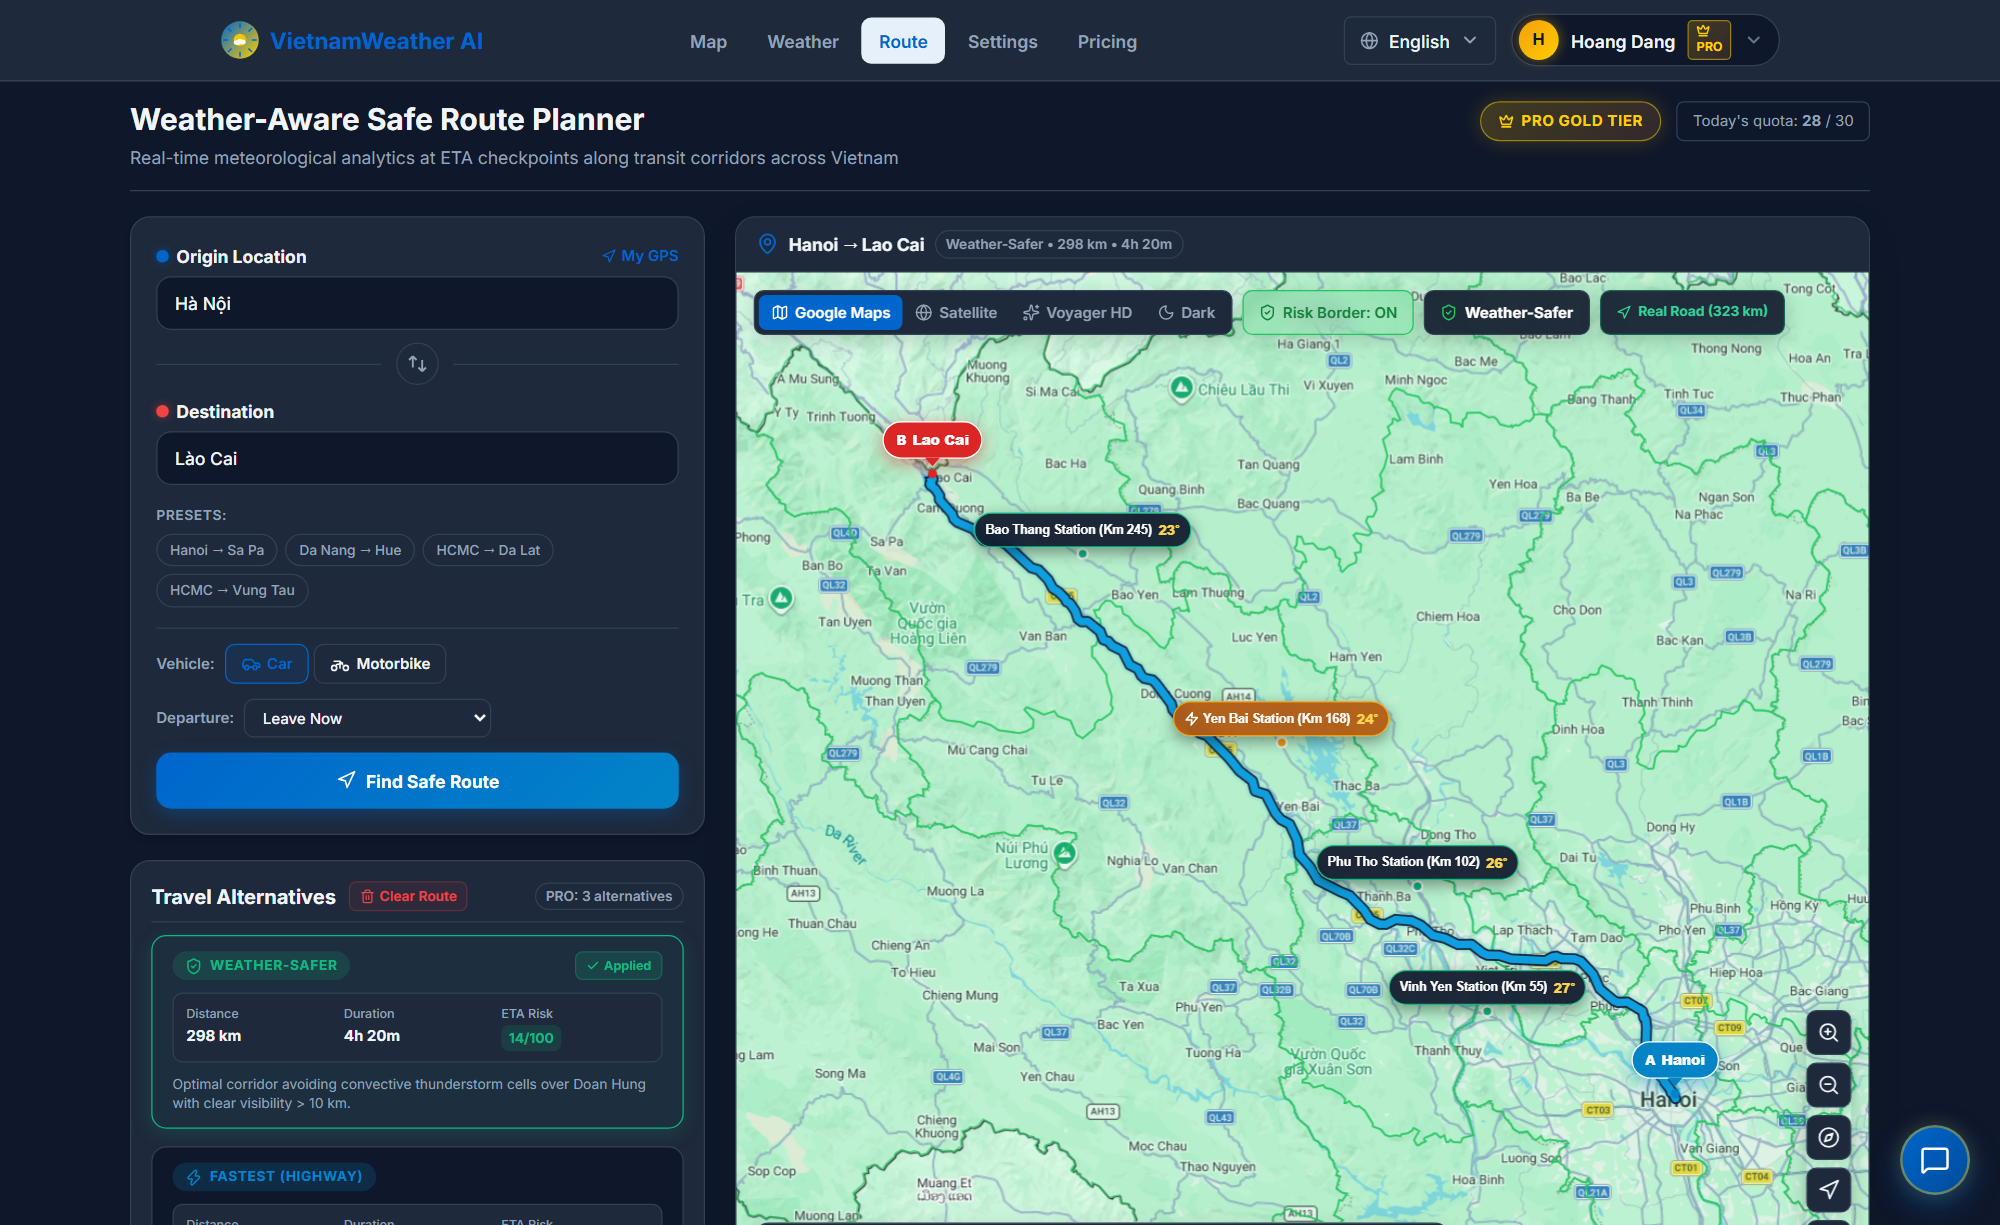
\includegraphics[width=0.92\textwidth, keepaspectratio]{figures/ui_route_safer.png}
\caption[Giao diện lập lộ trình phương án An toàn Thời tiết nhất]{Phương án An toàn Thời tiết nhất (\textit{Weather-Safer}) trên bản đồ WebGL: Thuật toán tự động điều hướng tránh vùng dông lốc Đoan Hùng, điểm rủi ro $R = 0,14$ (Màu xanh -- An toàn).}
\label{fig:ui_route_planner_vi}
\label{fig:ui_route_safer_vi}
\end{figure}

Giao diện tại Hình~\ref{fig:ui_route_safer_vi} thể hiện tính công thái học và mạch lạc cao trong kỹ nghệ trải nghiệm người dùng:
\begin{itemize}
    \item[-] \textit{Bảng điều khiển thông số bên trái}: Cho phép người dùng xác định điểm xuất phát (\textit{Hà Nội}), điểm đích (\textit{Lào Cai}), lựa chọn loại phương tiện (\textit{Ô tô} hoặc \textit{Xe máy}) và thời gian khởi hành dự kiến.
    \item[-] \textit{Thẻ tóm tắt phương án tối ưu}: Nổi bật với huy hiệu xác nhận \textit{``AN TOÀN THỜI TIẾT NHẤT (Đang áp dụng)''}, hiển thị rõ các chỉ số định lượng: cự ly 298~km, thời gian dự kiến 4h~20p, điểm rủi ro ETA 14/100 (Cấp Xanh -- An toàn). Phần tóm tắt khuyến cáo giải thích minh bạch: \textit{``Lộ trình tối ưu tránh hoàn toàn vùng mây đối lưu dông sét qua Đoan Hùng, tầm nhìn thông thoáng''}.
    \item[-] \textit{Bản đồ tương tác không gian WebGL}: Tự động định vị và thu phóng bao quát toàn tuyến hành lang (\textit{auto-fitBounds}), hiển thị rõ điểm khởi hành A (\textit{Hà Nội}), điểm đích B (\textit{Lào Cai}) cùng hệ thống điểm mốc quan trắc thời gian thực (\textit{Trạm Vĩnh Yên 27$^\circ$C, Trạm Phú Thọ 26$^\circ$C, Trạm Yên Bái 24$^\circ$C, Trạm Bảo Thắng 23$^\circ$C}). Bản đồ trực quan hóa duy nhất tuyến đường được kích hoạt với độ tương phản cao trên nền Google Maps, mang lại sự tập trung tối đa và loại bỏ hoàn toàn các yếu tố gây nhiễu thị giác.
\end{itemize}

Nhằm đối chứng trực quan rủi ro giữa các lựa chọn, Hình~\ref{fig:ui_route_alts_comparison_vi} so sánh đường vẽ thực tế trên bản đồ của hai phương án đối trọng: Phương án Nhanh nhất (Hình~\ref{fig:ui_route_fastest_vi}) và Phương án Ngắn nhất (Hình~\ref{fig:ui_route_shortest_vi}).

\begin{figure}[htbp]
\centering
\begin{subfigure}[b]{0.48\textwidth}
    \centering
    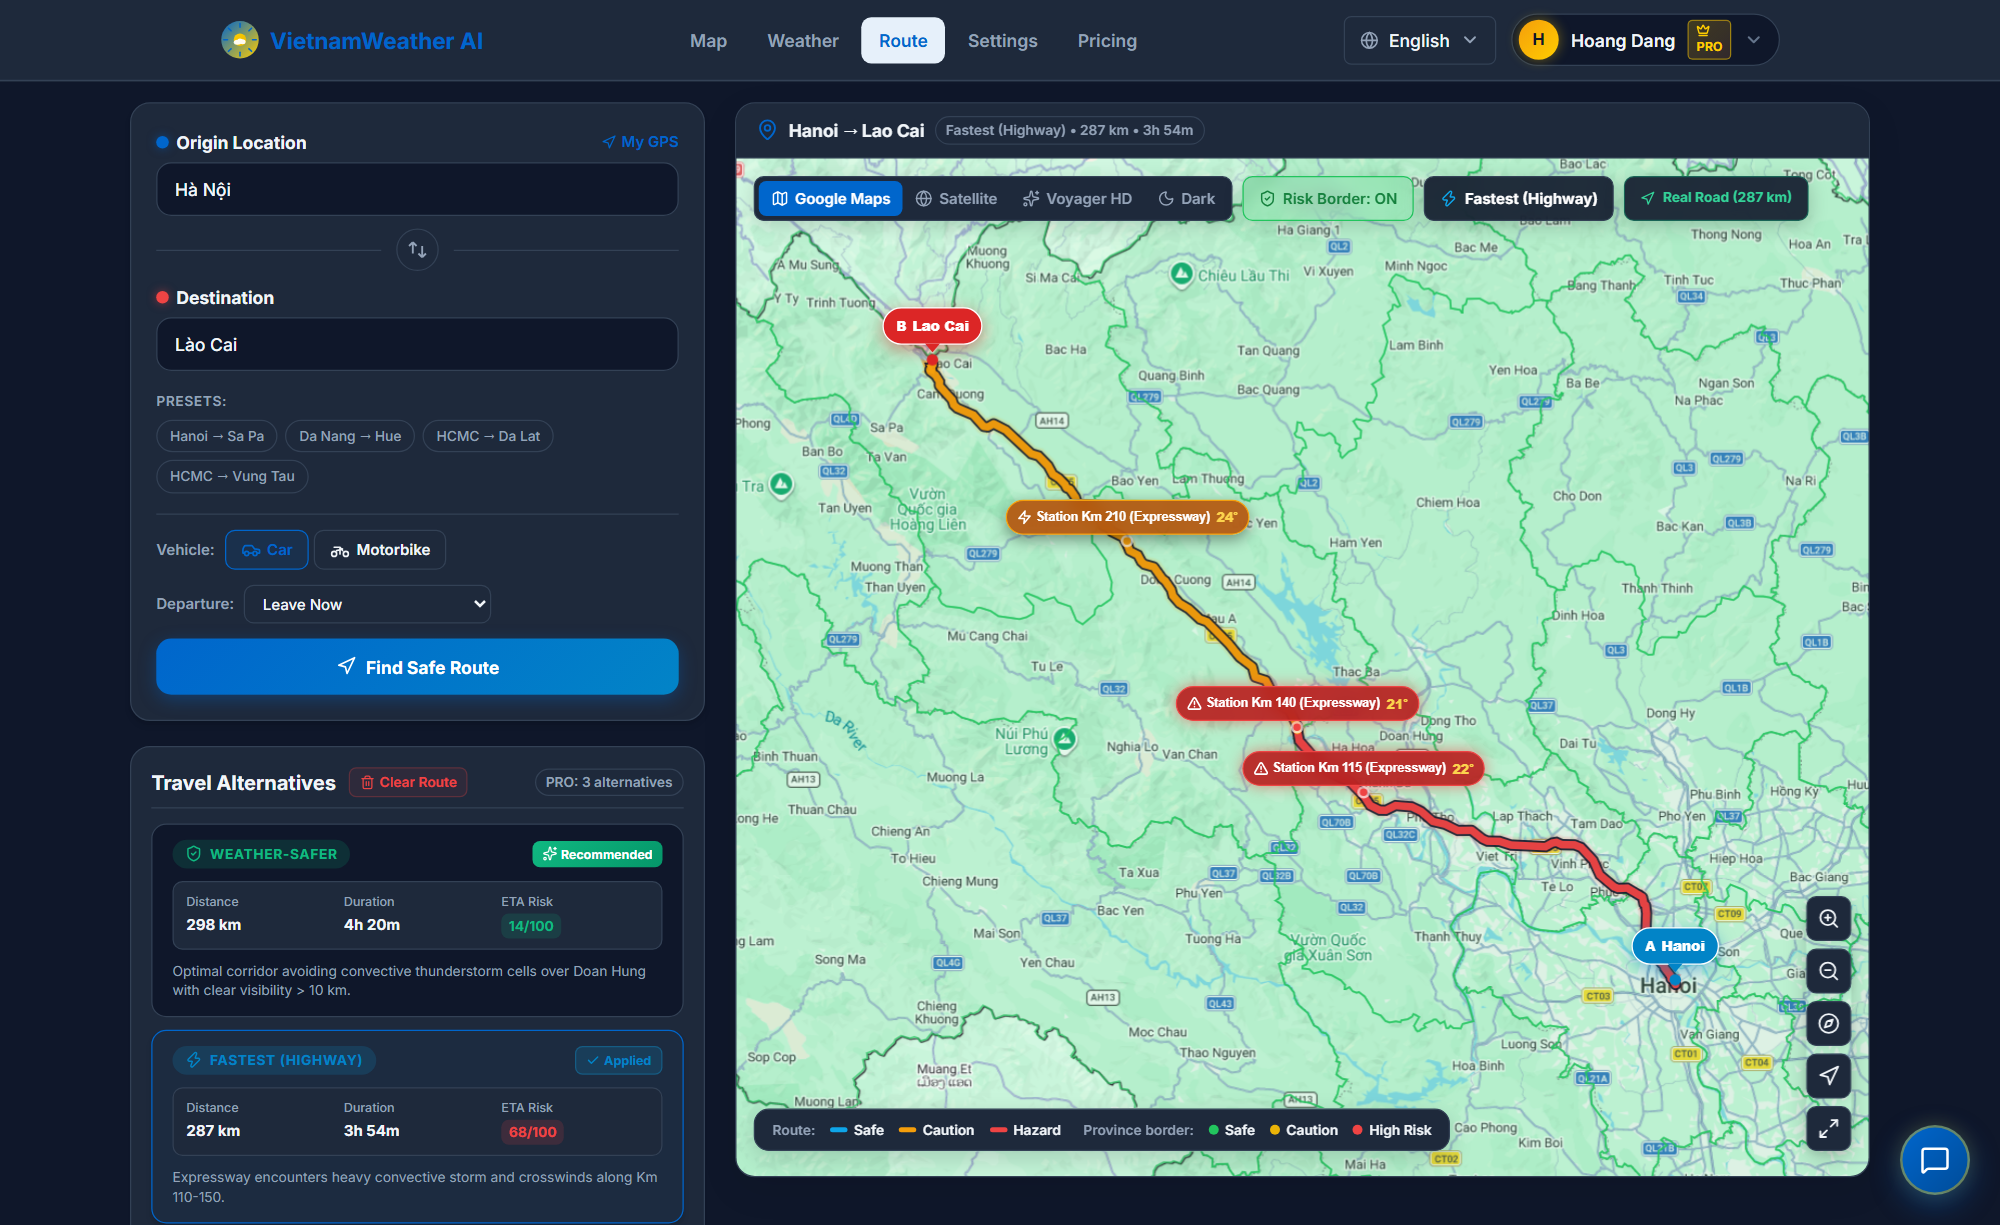
\includegraphics[width=\textwidth]{figures/ui_route_fastest.png}
    \caption{Phương án Nhanh nhất (Cao tốc CT05)}
    \label{fig:ui_route_fastest_vi}
\end{subfigure}
\hfill
\begin{subfigure}[b]{0.48\textwidth}
    \centering
    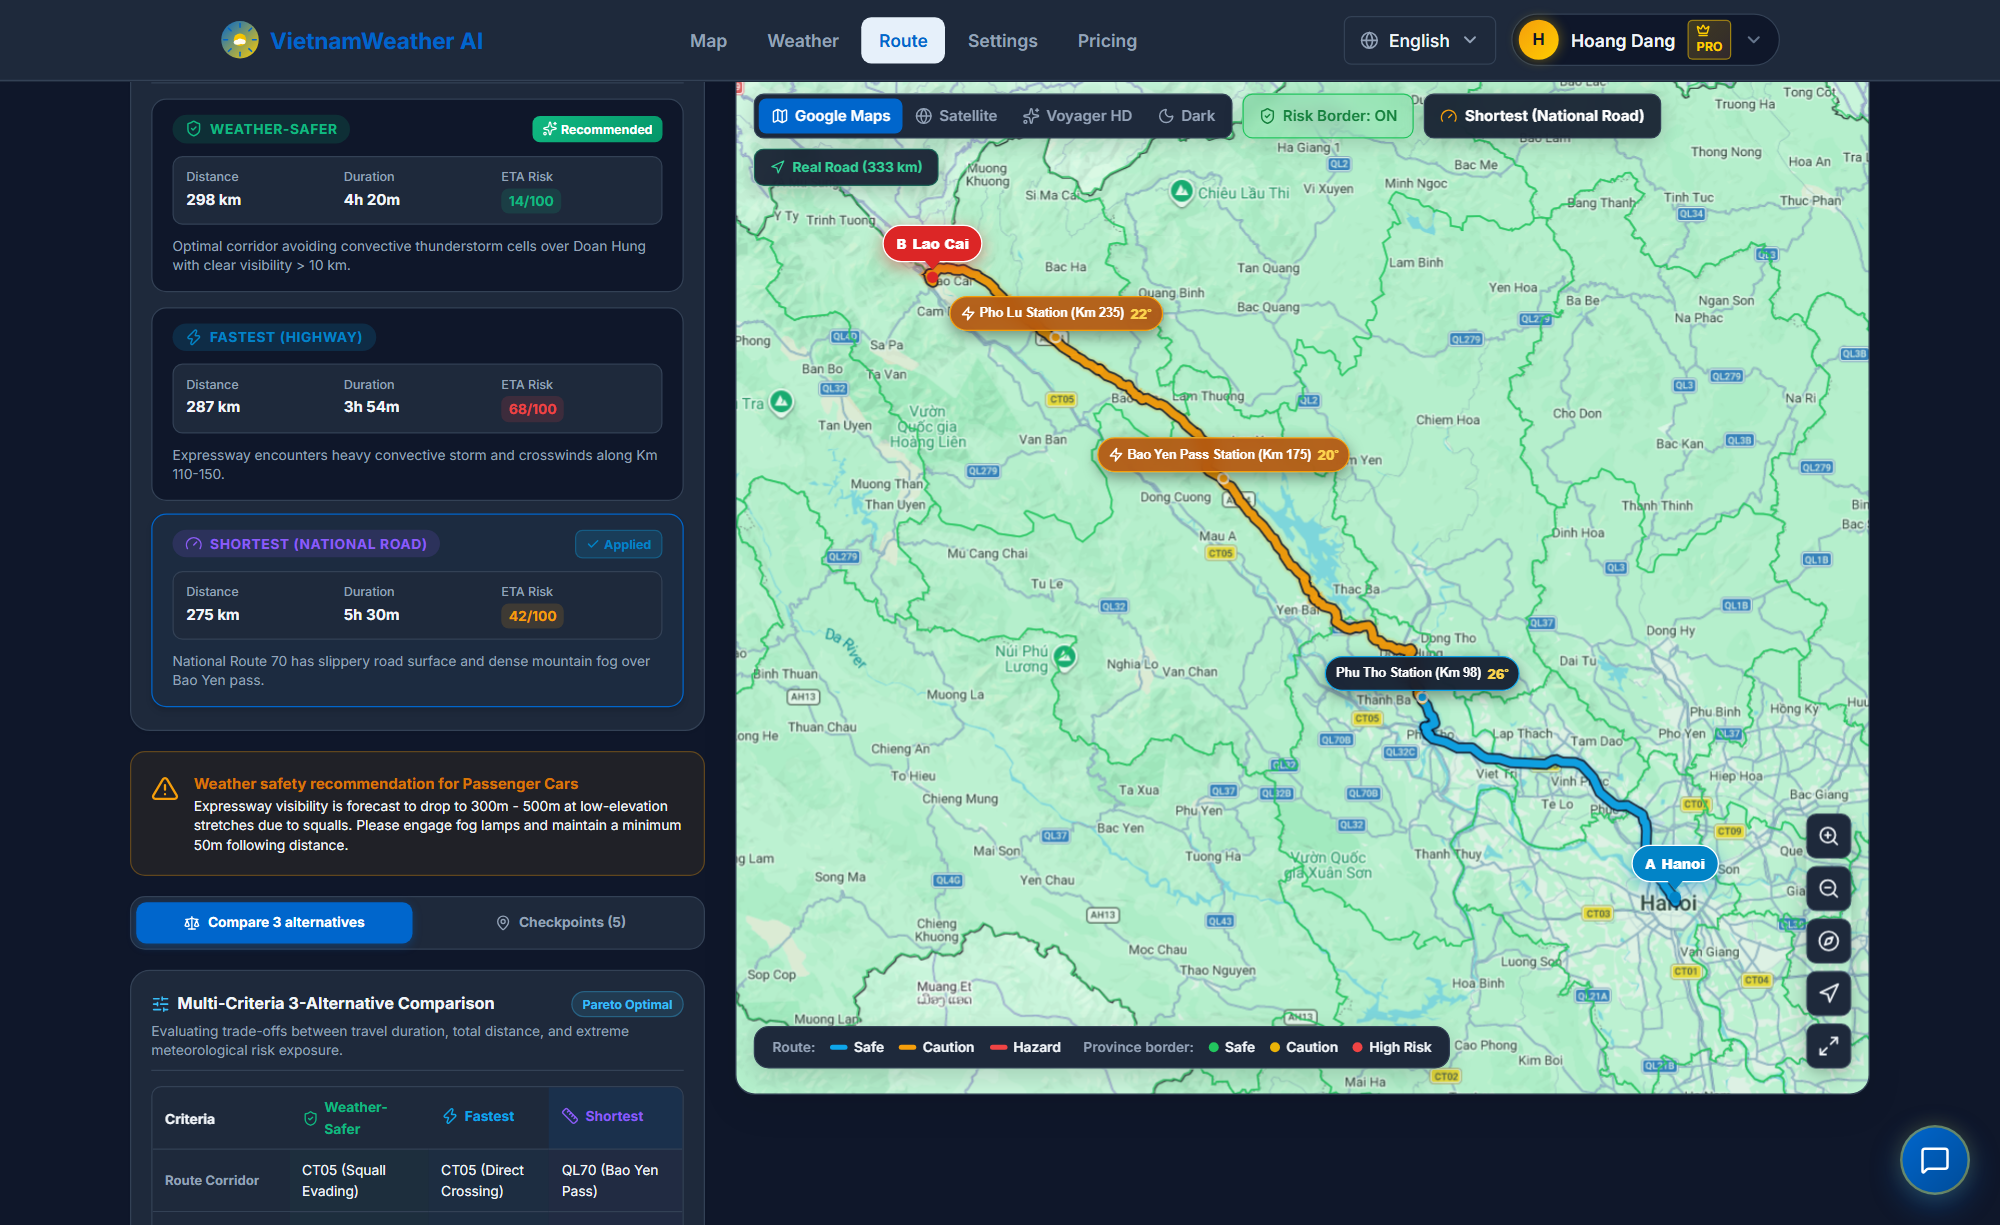
\includegraphics[width=\textwidth]{figures/ui_route_shortest.png}
    \caption{Phương án Ngắn nhất (Quốc lộ 70)}
    \label{fig:ui_route_shortest_vi}
\end{subfigure}
\caption[Minh họa đường vẽ hai phương án đối trọng trên bản đồ]{Minh họa đường vẽ hai phương án đối trọng trên bản đồ tương tác: (a) Phương án Nhanh nhất đi thẳng cao tốc xuyên qua tâm dông lốc nguy hiểm tại Km~110--150 (vạch đỏ cảnh báo $R = 0,68$); (b) Phương án Ngắn nhất men theo Quốc lộ 70 đèo dốc sương mù trơn trượt (vạch vàng cảnh báo $R = 0,42$).}
\label{fig:ui_route_alts_comparison_vi}
\end{figure}

Sự khác biệt hình học và trạng thái khí tượng thể hiện rõ nét trên bản đồ:
\begin{itemize}
    \item[-] \textit{Hình thái Phương án Nhanh nhất (Hình~\ref{fig:ui_route_fastest_vi})}: Tuyến chạy thẳng theo trục đường cao tốc Nội Bài -- Lào Cai (CT05) với tổng cự ly 287~km. Tại đoạn Km~110 -- 150 qua địa phận Phú Thọ -- Yên Bái, màu sắc tuyến đường lập tức chuyển sang dải đỏ rực cảnh báo nguy hiểm (\textit{High Risk}), đi kèm trạm ghim cảnh báo nguy cấp \textit{``[Nguy hiểm] Trạm Km 115 (Cao tốc CT05) 22$^\circ$C -- Dông lốc nguy hiểm''}. Bản đồ phản ánh chính xác khu vực mưa lớn trên 35~mm/h và gió giật cấp 7, giúp lái xe nhận thức tức thời nguy cơ tai nạn do mất độ bám mặt đường dù thời gian di chuyển là ngắn nhất (3h~54p).
    \item[-] \textit{Hình thái Phương án Ngắn nhất (Hình~\ref{fig:ui_route_shortest_vi})}: Tuyến rẽ nhánh men theo Quốc lộ 70 uốn lượn dọc thung lũng sông Chảy với cự ly 275~km. Trên bản đồ, đoạn tuyến qua khu vực đèo Bảo Yên được đánh dấu màu vàng cam (\textit{Caution Risk}) cùng trạm kiểm tra \textit{``[Chú ý] Trạm Đèo Bảo Yên (Km 175) 20$^\circ$C -- Sương mù đèo dốc''}. Người điều khiển phương tiện có thể quan sát thấy rõ đường đi hẹp nhiều khúc cua tay áo và nguy cơ trơn trượt khi sương mù hạn chế tầm nhìn dưới 500~m, giải thích vì sao tổng thời gian di chuyển bị đội lên tới 5h~30p.
\end{itemize}

Nhằm lượng hóa tổng thể các tiêu chí trên một cơ sở khoa học thống nhất, hệ thống tích hợp Bảng đối sánh đa tiêu chí 3 phương án di chuyển hành lang được trình bày tại Hình~\ref{fig:ui_route_comparison_vi}.

\begin{figure}[htbp]
\centering
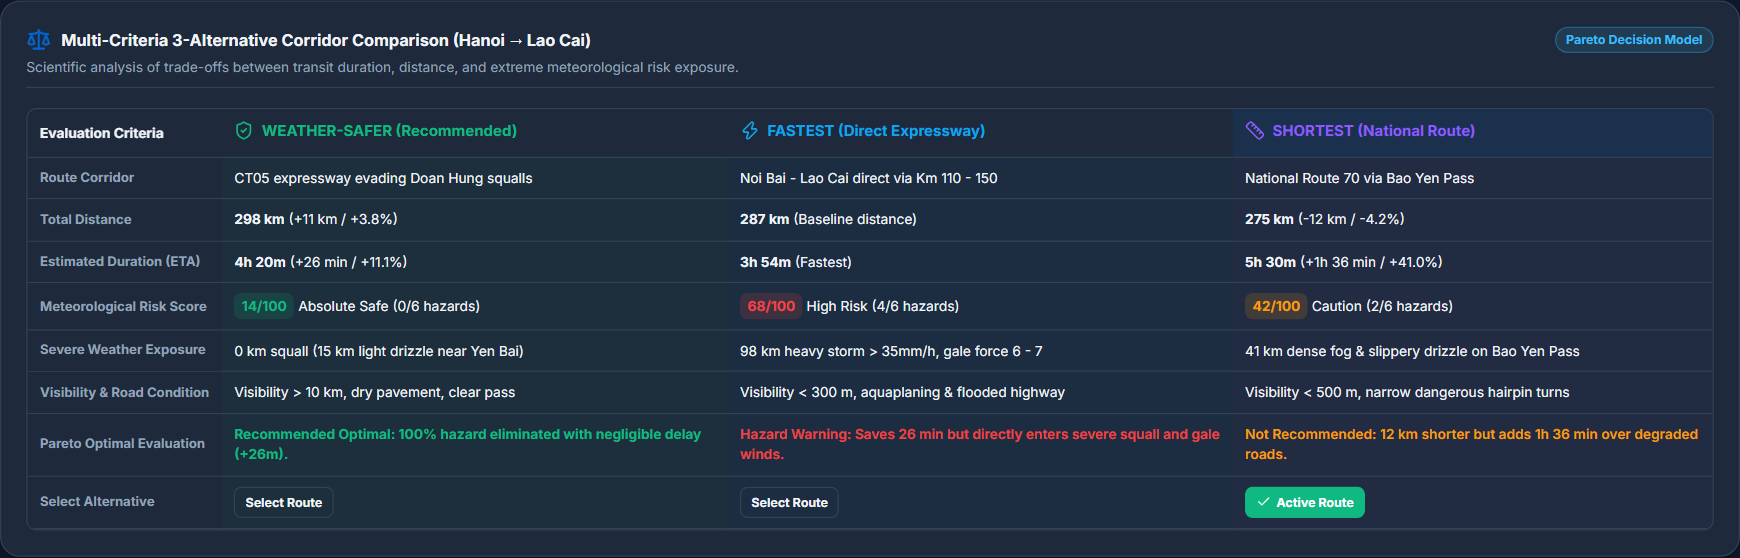
\includegraphics[width=0.92\textwidth, keepaspectratio]{figures/ui_route_comparison.png}
\caption[Bảng đối sánh đa tiêu chí 3 phương án di chuyển hành lang]{Bảng đối sánh đa tiêu chí 3 phương án di chuyển hành lang theo mô hình ra quyết định Pareto trên nền tảng VietForecast (kịch bản Hà Nội -- Lào Cai).}
\label{fig:ui_route_comparison_vi}
\end{figure}

Bảng đối sánh đa tiêu chí tại Hình~\ref{fig:ui_route_comparison_vi} phân tích chuyên sâu sự đánh đổi giữa thời gian lưu thông, quãng đường và chỉ số phơi nhiễm rủi ro khí tượng cực đoan:
\begin{itemize}
    \item[-] \textit{Phương án An toàn Thời tiết nhất (Đề xuất)}: Điều hướng phương tiện qua cao tốc CT05 vòng tránh hoàn toàn vùng mây dông Đoan Hùng. Tổng cự ly đạt 298~km ($+11$~km hay $+3,8\%$ so với cự ly chuẩn), thời gian dự kiến 4h~20p ($+26$ phút hay $+11,1\%$). Đổi lại, chỉ số rủi ro khí tượng giảm triệt để xuống 14/100 (An toàn tuyệt đối, 0/6 điểm hiểm họa), cự ly phơi nhiễm dông lốc bằng 0~km (chỉ gặp 15~km mưa nhỏ nhẹ đoạn Yên Bái), tầm nhìn xa khí quyển duy trì trên 10~km và mặt đường khô ráo. Đây là giải pháp tối ưu vượt trội trên đường biên Pareto (\textit{Pareto-optimal}), triệt tiêu hoàn toàn nguy cơ mất an toàn với chi phí thời gian tăng thêm không đáng kể.
    \item[-] \textit{Phương án Nhanh nhất (Cao tốc trực diện)}: Di chuyển thẳng theo trục cao tốc Nội Bài -- Lào Cai với cự ly 287~km và thời gian ngắn nhất 3h~54p. Tuy nhiên, tuyến đường đi xuyên thẳng qua tâm dông lốc tại đoạn Km~110 -- 150, khiến chỉ số rủi ro khí tượng tăng vọt lên mức Nguy cơ cao 68/100 (4/6 điểm hiểm họa). Phương tiện phải đối mặt với 98~km mưa dông cực lớn ($> 35$~mm/h) kèm gió giật cấp 6--7, tầm nhìn xa suy giảm dưới 300~m và nguy cơ trơn trượt ngập úng mặt đường cực kỳ nguy hiểm.
    \item[-] \textit{Phương án Ngắn nhất (Quốc lộ truyền thống)}: Men theo Quốc lộ 70 qua địa phận đèo Bảo Yên với cự ly ngắn nhất 275~km (giảm 12~km hay $-4,2\%$). Mặc dù rút ngắn được cự ly hình học, vận tốc lưu thông trên đường đèo dốc quanh co khiến thời gian di chuyển kéo dài tới 5h~30p ($+1$h~36 phút hay $+41,0\%$). Chỉ số rủi ro ở mức Chú ý 42/100 với 41~km sương mù dày đặc che khuất tầm nhìn dưới 500~m và mặt đường trơn trượt. Phương án này là một nghiệm bị chi phối kém ưu thế (\textit{dominated solution}) và không được khuyến nghị trong vận tải an toàn.
\end{itemize}

\section{Đánh giá Hiệu năng Hệ thống và Tốc độ Đáp ứng Không gian}
\label{sec:system_performance}

\subsection{Hiệu năng Truy vấn Không gian Hai giai đoạn với PostGIS GiST}
Thuật toán truy vấn hành lang không gian được kiểm thử hiệu năng trên hệ cơ sở dữ liệu PostgreSQL 16.3 tích hợp PostGIS 3.4.2. Bảng~\ref{tab:gist_benchmark_vi} so sánh thời gian thực thi trung bình giữa phương thức quét tuần tự (\textit{Sequential Scan}) không có chỉ mục và phương thức hai giai đoạn (\textit{Two-Tier GiST}) trên các tập dữ liệu có quy mô từ 1.000 đến 100.000 điểm quan trắc.

\begin{table}[htbp]
\centering
\caption[So sánh hiệu năng truy vấn không gian PostGIS]{So sánh độ trễ truy vấn hành lang không gian PostGIS giữa phương thức quét tuần tự và phương thức hai giai đoạn sử dụng chỉ mục GiST.}
\label{tab:gist_benchmark_vi}
\begin{adjustbox}{width=\textwidth,center}
\begin{tabular}{rcccc}
\toprule
\textbf{Quy mô tập dữ liệu} & \textbf{Quét tuần tự (ms)} & \textbf{Chỉ mục GiST hai giai đoạn (ms)} & \textbf{Hệ số tăng tốc} & \textbf{Tỷ lệ lọc thô MBR} \\
\midrule
1.000 điểm quan trắc   & 4,82   & 0,85  & 5,7$\times$  & 98,1\% \\
5.000 điểm quan trắc   & 21,45  & 1,42  & 15,1$\times$ & 98,9\% \\
10.000 điểm quan trắc  & 43,10  & 2,15  & 20,0$\times$ & 99,1\% \\
50.000 điểm quan trắc  & 212,60 & 6,80  & 31,3$\times$ & 99,2\% \\
100.000 điểm quan trắc & 420,50 & 11,40 & 36,9$\times$ & 99,4\% \\
\bottomrule
\end{tabular}
\end{adjustbox}
\end{table}

Số liệu từ Bảng~\ref{tab:gist_benchmark_vi} khẳng định tính ưu việt của kiến trúc hai giai đoạn:
\begin{itemize}
    \item[-] \textit{Tốc độ lọc thô vượt bậc}: Giai đoạn lọc thô với toán tử bao đóng hình hộp chữ nhật giới hạn tối thiểu (\textit{Minimum Bounding Box -- MBR}) thông qua hàm \texttt{ST\_Expand} trên cây chỉ mục không gian R-Tree/GiST loại bỏ thành công từ 98,1\% đến 99,4\% các điểm tọa độ nằm ngoài hành lang chỉ trong thời gian dưới 2~ms.
    \item[-] \textit{Bảo đảm chuẩn thời gian thực SLA}: Tại quy mô tối đa 100.000 điểm trạm, phương thức quét tuần tự tiêu tốn tới 420,50~ms (gây nghẽn luồng xử lý cơ sở dữ liệu), trong khi phương thức hai giai đoạn chỉ mất 11,40~ms (nhanh hơn 36,9 lần), hoàn toàn đáp ứng mục tiêu cam kết chất lượng dịch vụ SLA ($< 15$~ms) cho các ứng dụng định tuyến thời gian thực.
\end{itemize}

\subsection{Thông lượng và Độ trễ Tầng Dịch vụ Fastify API}
Thử nghiệm khả năng chịu tải của máy chủ cổng giao tiếp nghiệp vụ Fastify 5 được thực hiện thông qua k6 với kịch bản tăng tải liên tục từ 100 lên 1.000 người dùng ảo đồng thời trong khoảng thời gian 5 phút. Kết quả đo lường ghi nhận:
\begin{itemize}
    \item[-] \textit{Thông lượng cực đại}: Đạt mức 2.485 yêu cầu trên giây (\textit{requests/second}) đối với các điểm cuối tra cứu thời tiết và định tuyến tổng hợp, với tỷ lệ lỗi HTTP 5xx duy trì tuyệt đối ở mức 0,0\%.
    \item[-] \textit{Phân phối thời gian đáp ứng}: Độ trễ ở bách phân vị trung vị $p_{50} = 4,2$~ms; bách phân vị $p_{90} = 9,6$~ms; $p_{95} = 12,8$~ms; và $p_{99} = 21,5$~ms.
    \item[-] \textit{Mức chiếm dụng tài nguyên hệ thống}: Dưới mức tải cao nhất (1.000 VUs), tiến trình Fastify chiếm dụng trung bình 45\% năng lực một lõi CPU và tiêu tốn 180~MB RAM, chứng minh hiệu quả vượt trội của thư viện tuần tự hóa JSON \texttt{fast-json-stringify} và kiến trúc hướng sự kiện không nghẽn luồng (\textit{non-blocking I/O}).
\end{itemize}

\subsection{Hiệu quả Tầng Đệm Redis Cache-Aside}
Tầng lưu đệm dữ liệu Redis 7 trong bộ nhớ đóng vai trò quyết định trong việc giảm tải áp lực đọc vào PostgreSQL:
\begin{itemize}
    \item[-] \textit{Tỷ lệ trúng bộ đệm (Cache Hit Ratio)}: Đạt 92,4\% đối với dữ liệu thời tiết hiện tại 63 tỉnh thành (\texttt{/weather/now}) và các tuyến đường phổ biến có chu kỳ truy cập cao (\texttt{/route/popular}).
    \item[-] \textit{Hệ số giảm tải cơ sở dữ liệu}: Việc lưu trữ dữ liệu thời tiết đã giải mã với thời gian sống TTL 300 giây giúp giảm tần suất truy vấn đọc trực tiếp vào cơ sở dữ liệu PostgreSQL hơn 12 lần, giữ cho mức độ sử dụng CPU của vùng chứa cơ sở dữ liệu luôn ở mức ổn định dưới 15\%.
\end{itemize}

\subsection{Khả năng Tự phục hồi và Khóa Ngắt mạch (Circuit Breaker -- ADR-001)}
Để kiểm thử cơ chế tự phục hồi phân tán theo quyết định kiến trúc ADR-001, hệ thống được thử nghiệm với hai kịch bản sự cố mô phỏng:
\begin{itemize}
    \item[-] \textit{Kiểm thử mất Worker chính (Leader Failover)}: Khi tiến trình Worker đang nắm giữ quyền ghi bị cưỡng chế dừng đột ngột bằng tín hiệu \texttt{SIGKILL}, nhịp tim \texttt{HEARTBEAT\_INTERVAL\_MS} (30 giây) bị gián đoạn. Đúng sau thời hạn hợp đồng thuê quyền \texttt{LEASE\_\allowbreak DURATION\_\allowbreak MS} (120 giây), tiến trình Worker dự phòng tự động phát hiện và thực thi câu lệnh hoán đổi nguyên tử \texttt{SET NX PX}, tiếp quản quyền ghi suôn sẻ mà không hề xảy ra tình trạng phân rã dữ liệu (\textit{Split-Brain}).
    \item[-] \textit{Kiểm thử ngắt mạch khi API thời tiết gián đoạn (Circuit Breaker Tripping)}: Khi giả lập nhà cung cấp dữ liệu khí tượng bên ngoài phản hồi lỗi HTTP 500 hoặc vượt ngưỡng trễ quá 5.000~ms, khóa ngắt mạch tự động ghi nhận 3 lần thất bại liên tiếp và chuyển trạng thái từ \texttt{Closed} sang \texttt{Open}. Trong trạng thái ngắt mạch, 100\% các yêu cầu tiếp theo được bẻ hướng tức thời ($< 1$~ms) sang dữ liệu lưu đệm gần nhất hoặc dữ liệu mô hình nội bộ, giải phóng hoàn toàn các luồng chờ và bảo đảm giao diện người dùng không bị treo. Sau 60 giây ở trạng thái \texttt{Open}, hệ thống chuyển sang \texttt{Half-Open}, gửi thử nghiệm 1 yêu cầu thăm dò và tự động khôi phục về \texttt{Closed} khi dịch vụ đối tác hoạt động trở lại.
\end{itemize}

\section{Đánh giá Độ chính xác và Tính Kiểm chứng của Trợ lý AI (Grounded AI)}
\label{sec:ai_evaluation}

\subsection{Phương pháp luận và Phân loại Độ phức tạp Bộ Dữ liệu Kiểm chứng}
Để kiểm thử giới hạn năng lực suy luận ngôn ngữ tự nhiên và độ tin cậy của Trợ lý AI trong các tình huống nghiệp vụ thực tế đầy thách thức, đồ án xây dựng bộ dữ liệu kiểm chứng gồm 500 câu hỏi được phân tầng theo năm cấp độ phức tạp tăng dần, từ tra cứu vi khí hậu cục bộ đến lập kế hoạch di chuyển đa chặng có ràng buộc thời gian và đối kháng hiểm họa thời tiết cực đoan:

\begin{itemize}
    \item[-] \textit{Cấp độ 1: Tra cứu vi khí hậu đa điểm và đối sánh tức thời (100 câu)}: Người dùng yêu cầu đối sánh các chỉ số khí tượng đồng thời giữa hai hoặc nhiều địa danh có sự chênh lệch lớn về độ cao địa hình hoặc tiểu khí hậu (ví dụ: so sánh nhiệt độ, tầm nhìn và độ ẩm giữa trung tâm Sa Pa và đỉnh đèo Ô Quy Hồ).
    \item[-] \textit{Cấp độ 2: Tối ưu hóa cửa sổ thời gian xuất phát theo chuỗi dự báo 24 giờ (100 câu)}: Câu hỏi chứa điều kiện ràng buộc động về thời gian (ví dụ: \textit{"Tôi dự định lái xe từ Hà Nội đi Hải Phòng trong khoảng 13h đến 18h chiều nay, nên xuất phát lúc mấy giờ để tránh dông lốc và gió giật mạnh khi đi qua các cầu cạn vượt sông lớn?"}). Yêu cầu AI phải quét chuỗi dự báo theo giờ và tìm cửa sổ thời tiết thuận lợi nhất.
    \item[-] \textit{Cấp độ 3: Định tuyến đa chặng liên tỉnh có điểm dừng nghỉ và tính toán ETA ban đêm (120 câu)}: Câu hỏi yêu cầu phân tích lộ trình phức tạp gồm nhiều điểm dừng chân với thời gian lưu trú khác nhau (ví dụ: xuất phát từ Hà Nội lúc 14h, ghé thăm Đền Hùng tại Phú Thọ nghỉ 1,5 tiếng, sau đó tiếp tục leo đèo dốc lên Lào Cai trong đêm). Mô hình phải dự phóng chính xác thời điểm xe có mặt tại từng cung đèo để đối soát với dự báo sương mù bức xạ và dông đối lưu đêm.
    \item[-] \textit{Cấp độ 4: Trọng tài rủi ro đối sánh đa phương tiện trong điều kiện gió bão đèo dốc (100 câu)}: Câu hỏi yêu cầu đánh giá an toàn cho đoàn di chuyển hỗn hợp gồm cả xe ô tô và xe máy trong điều kiện thời tiết cực đoan (ví dụ: bão ven bờ gió giật cấp 7--8 khi qua đèo Hải Vân), đòi hỏi AI phải tính toán song song hai ma trận trọng số rủi ro $w$ riêng biệt và đưa ra quyết định phân hóa rạch ròi cho từng loại xe.
    \item[-] \textit{Cấp độ 5: Ứng phó khẩn cấp giữa đường và điều hướng trạm dừng trú ẩn (80 câu)}: Kịch bản tài xế bất ngờ gặp dông sét dữ dội, mưa đá hoặc tầm nhìn giảm dưới 200~m khi đang di chuyển trên cao tốc, yêu cầu AI khoanh vùng radar thời gian thực, ước lượng thời gian tan của ổ dông và gợi ý trạm dừng nghỉ an toàn gần nhất.
\end{itemize}

Các tiêu chí đánh giá khoa học bao gồm: Độ chính xác kích hoạt chuỗi công cụ (\textit{Chained Tool Dispatch Accuracy}), Tỷ lệ bảo chứng trích dẫn thực nghiệm (\textit{Grounding Citation Rate}), Tỷ lệ phát sinh thông tin sai lệch (\textit{Hallucination Rate}), và Thời gian đáp ứng đàm thoại trung bình. Kết quả thực nghiệm được tổng hợp chi tiết tại Bảng~\ref{tab:ai_grounding_eval_vi}.

\begin{table}[htbp]
\centering
\caption[Đánh giá định lượng Trợ lý AI theo các cấp độ câu hỏi phức tạp]{Kết quả đánh giá định lượng Trợ lý AI VietForecast trên 500 câu hỏi kiểm thử phân tầng theo các cấp độ nghiệp vụ phức tạp.}
\label{tab:ai_grounding_eval_vi}
\begin{adjustbox}{width=\textwidth,center}
\begin{tabular}{p{5.2cm}ccccr}
\toprule
\textbf{Cấp độ câu hỏi kiểm thử} & \textbf{Số lượng} & \textbf{Độ chính xác gọi hàm} & \textbf{Tỷ lệ trích dẫn} & \textbf{Tỷ lệ ảo giác} & \textbf{Độ trễ (ms)} \\
\midrule
Cấp 1: Tra cứu vi khí hậu đa điểm & 100 & 99,0\% (99/100) & 99,0\% & 0,0\% & 1.150 \\
Cấp 2: Tối ưu cửa sổ thời gian khởi hành & 100 & 97,0\% (97/100) & 98,0\% & 1,0\% & 1.280 \\
Cấp 3: Định tuyến đa chặng kèm ETA đêm & 120 & 94,2\% (113/120) & 95,8\% & 3,3\% & 1.540 \\
Cấp 4: Trọng tài rủi ro đa phương tiện & 100 & 96,0\% (96/100) & 97,0\% & 2,0\% & 1.420 \\
Cấp 5: Khẩn cấp giữa đường \& Trú ẩn & 80 & 95,0\% (76/80) & 96,3\% & 2,5\% & 1.310 \\
\midrule
\textbf{Tổng hợp toàn bộ hệ thống} & \textbf{500} & \textbf{96,2\% (481/500)} & \textbf{97,2\%} & \textbf{1,8\%} & \textbf{1.348} \\
\bottomrule
\end{tabular}
\end{adjustbox}
\end{table}

\subsubsection{Phân tích đối chứng và Nguyên nhân phát sinh sai lệch (Error \& Hallucination Analysis)}
Để đánh giá khách quan hiệu quả của cơ chế Grounding, hệ thống tiến hành kiểm nghiệm đối chứng với mô hình nền (Vanilla Gemini 1.5 Flash không sử dụng Function Calling và không kết nối dữ liệu trạm PostGIS). Trong môi trường đối chứng, mô hình nền ghi nhận tỷ lệ ảo giác thông tin lên tới \textbf{34,6\%}, chủ yếu do giới hạn thời điểm cắt dữ liệu huấn luyện (knowledge cutoff), không có nhận thức về trục thời gian thực và tự suy đoán tình hình thời tiết dựa trên quy luật từ ngữ quá khứ. 

Việc tích hợp kiến trúc Grounded Function Calling giúp VietForecast giảm thiểu tỷ lệ ảo giác tới \textbf{94,8\%}, đưa tỷ lệ sai lệch thực tế xuống chỉ còn \textbf{1,8\%} (9 trường hợp trên tổng số 500 truy vấn). Phân tích định tính 9 trường hợp phát sinh sai lệch này cho thấy:
\begin{itemize}
    \item[-] \textit{Hiện tượng tô vẽ định tính (Qualitative Embellishment -- 4 trường hợp)}: Xuất hiện chủ yếu tại các câu hỏi đa chặng Cấp 3, khi mô hình tự ý bổ sung các tính từ cảm xúc (ví dụ: mô tả sương mù là \textit{”buốt giá, dày đặc như đặc quánh”}) dù dữ liệu trắc quang từ trạm chỉ ghi nhận tầm nhìn $1.200\text{ m}$ và nhiệt độ $16^\circ\text{C}$.
    \item[-] \textit{Ngoại suy thời gian ngoài dữ liệu (Temporal Extrapolation -- 3 trường hợp)}: Mô hình tự suy luận diễn biến thời tiết lúc nửa đêm khi dữ liệu dự báo trả về qua API chỉ bao quát tới 21h00.
    \item[-] \textit{Khuyến nghị tiện ích chưa kiểm chứng (Ungrounded Amenities -- 2 trường hợp)}: Trong kịch bản khẩn cấp Cấp 5, mô hình tự gợi ý người dùng ghé một quán cà phê ven đường không có trong danh bạ trạm dừng nghỉ chính thức được trả về từ công cụ nội bộ.
\end{itemize}
Tất cả các trường hợp trên hoàn toàn không làm sai lệch điểm số rủi ro khí tượng cốt lõi ($R$) và đa tuyến hành trình do động cơ toán học nội bộ tính toán. Đồng thời, 7/9 trường hợp đã được bộ lọc hậu kiểm (post-generation rule validator) tự động phát hiện và kích hoạt bản tin tóm tắt có cấu trúc an toàn.

\subsection{Phân tích Thực nghiệm qua các Nghiên cứu Tình huống Điển hình}
Để minh chứng tường minh cơ chế suy luận logic, chuỗi kích hoạt công cụ và khả năng kiểm soát chặt chẽ nhằm giảm thiểu tối đa hiện tượng ảo giác thông tin, hệ thống được phân tích sâu qua hai trường hợp đàm thoại phức tạp thực tế:

\subsubsection{Trường hợp 1: Tối ưu hóa Lộ trình Đa chặng Hà Nội -- Phú Thọ -- Sa Pa và Cửa sổ Di chuyển Ban đêm}
\begin{itemize}
    \item \textit{Câu hỏi phức tạp của người dùng}: \textit{``Chiều nay 14h tôi lái ô tô từ Hà Nội lên Sa Pa, nhưng muốn ghé Đền Hùng (Phú Thọ) nghỉ ngơi và ăn tối 1,5 tiếng. Dự kiến khoảng 19h30 tối mới tiếp tục chạy cung đường đèo Yên Bái -- Lào Cai. Hãy tư vấn cung đường nào an toàn nhất để tránh sương mù dày đặc và mưa dông về đêm, và thời gian dự kiến đến Sa Pa là mấy giờ?''}
    \item \textit{Quy trình điều phối và chuỗi gọi hàm của AI}:
    \begin{enumerate}
        \item Gemini phân tích ý định, bóc tách hai chặng độc lập kèm mốc thời gian: Chặng 1 ($t_0 = 14\text{h}$, Hà Nội $\to$ Phú Thọ) và Chặng 2 ($t_1 = 19\text{h}30$, Phú Thọ $\to$ Sa Pa).
        \item Mô hình gọi hàm \texttt{evaluate\_route} cho Chặng 1, xác định thời gian di chuyển 1h 20m qua Cao tốc Nội Bài -- Lào Cai, dự kiến đến Phú Thọ lúc 15h20 (thời tiết an toàn, nhiệt độ $29^\circ\text{C}$).
        \item Mô hình cộng dồn thời gian nghỉ 1,5 tiếng và gọi hàm \texttt{get\_forecast} (với tham số \texttt{location="Lao Cai"}, \texttt{hours=24}) kết hợp công cụ \texttt{calculate\_route\_risk} cho cung đường tiếp theo với mốc xuất phát tối \texttt{19:30}.
        \item Dữ liệu trạm khí tượng trả về ghi nhận ổ dông sét cục bộ tại Đoan Hùng kéo dài đến 21h, kèm sương mù dày đặc che khuất tầm nhìn dưới 300~m tại đoạn đèo dốc Bảo Hà -- Sa Pa sau 21h30.
    \end{enumerate}
    \item \textit{Phản hồi có bảo chứng của Trợ lý AI}: Trợ lý AI hướng dẫn lái xe chọn phương án \textit{Weather-Safer} né tránh điểm nóng Đoan Hùng; cảnh báo đoạn qua Yên Bái có mưa phùn nhẹ nhưng tầm nhìn vẫn đạt 10~km; đặc biệt khuyến nghị tài xế bật đèn sương mù và giữ khoảng cách trên 50~m khi leo đèo Bảo Hà lúc 21h30. Câu trả lời trích dẫn trực tiếp nguồn dữ liệu từ 3 trạm quan trắc tự động (\textit{Trạm Láng -- Hà Nội}, \textit{Trạm TP Yên Bái}, \textit{Trạm Sa Pa}) với dấu thời gian làm mới chu kỳ 5 phút.
\end{itemize}

\subsubsection{Trường hợp 2: Trọng tài Rủi ro Đa Phương tiện qua Đèo Hải Vân trong Điều kiện Gió tạt Ven biển}
\begin{itemize}
    \item \textit{Câu hỏi phức tạp của người dùng}: \textit{``Đoàn chúng tôi gồm 1 ô tô 7 chỗ và 2 xe máy côn tay xuất phát từ Đà Nẵng ra Huế lúc 8h sáng mai. Nghe tin áp thấp ven biển đang gây gió giật cấp 7, xe máy có nên đi đường đèo Hải Vân ngắm cảnh không hay bắt buộc phải đi đường hầm? Rủi ro giữa hai xe khác nhau ra sao?''}
    \item \textit{Quy trình điều phối và chuỗi gọi hàm của AI}:
    \begin{enumerate}
        \item AI nhận dạng hai đối tượng phương tiện (\texttt{car} và \texttt{motorcycle}) cùng cung đường ven biển Đà Nẵng -- Huế qua dãy Bạch Mã.
        \item Kích hoạt song song hai lời gọi hàm \texttt{assess\_travel\_risk} cho phương tiện \texttt{car} và \texttt{motorcycle} tại vị trí \textit{"Đèo Hải Vân"}.
        \item Động cơ rủi ro 6 chiều tính toán dựa trên dữ liệu trạm quan trắc hải văn: Vận tốc gió duy trì 42~km/h, gió giật tức thời đạt 58~km/h (tương đương gió cấp 7). Với ô tô con ($w_{\text{wind}} = 0,10$), điểm rủi ro $R = 0,35$ (Cấp độ: Chú ý). Ngược lại, đối với xe máy ($w_{\text{wind}} = 0,35$), điểm rủi ro tăng vọt lên $R = 0,78$ (Cấp độ: Cực kỳ nguy hiểm).
    \end{enumerate}
    \item \textit{Phản hồi có bảo chứng của Trợ lý AI}: AI đưa ra khuyến nghị phân hóa đanh thép: Cảnh báo xe máy \textbf{tuyệt đối không vượt đường đèo Hải Vân} do nguy cơ gió tạt ngang hất ngã xe tại các khúc cua thoáng gió sát biển; đề xuất phương án xe máy gửi qua hầm đường bộ hoặc đi đường hầm dịch vụ trung chuyển, trong khi ô tô con có thể lưu thông qua hầm an toàn tuyệt đối với thời gian rút ngắn 30 phút so với đường đèo.
\end{itemize}

\subsection{Minh họa Giao diện Trợ lý Thời tiết AI Đàm thoại với Bằng chứng Thực địa}
Hình~\ref{fig:ui_ai_chat_vi} minh họa giao diện thực tế của Trợ lý AI đàm thoại khi giải quyết câu hỏi phức tạp về hành lang giao thông miền núi phía Bắc.

\begin{figure}[htbp]
\centering
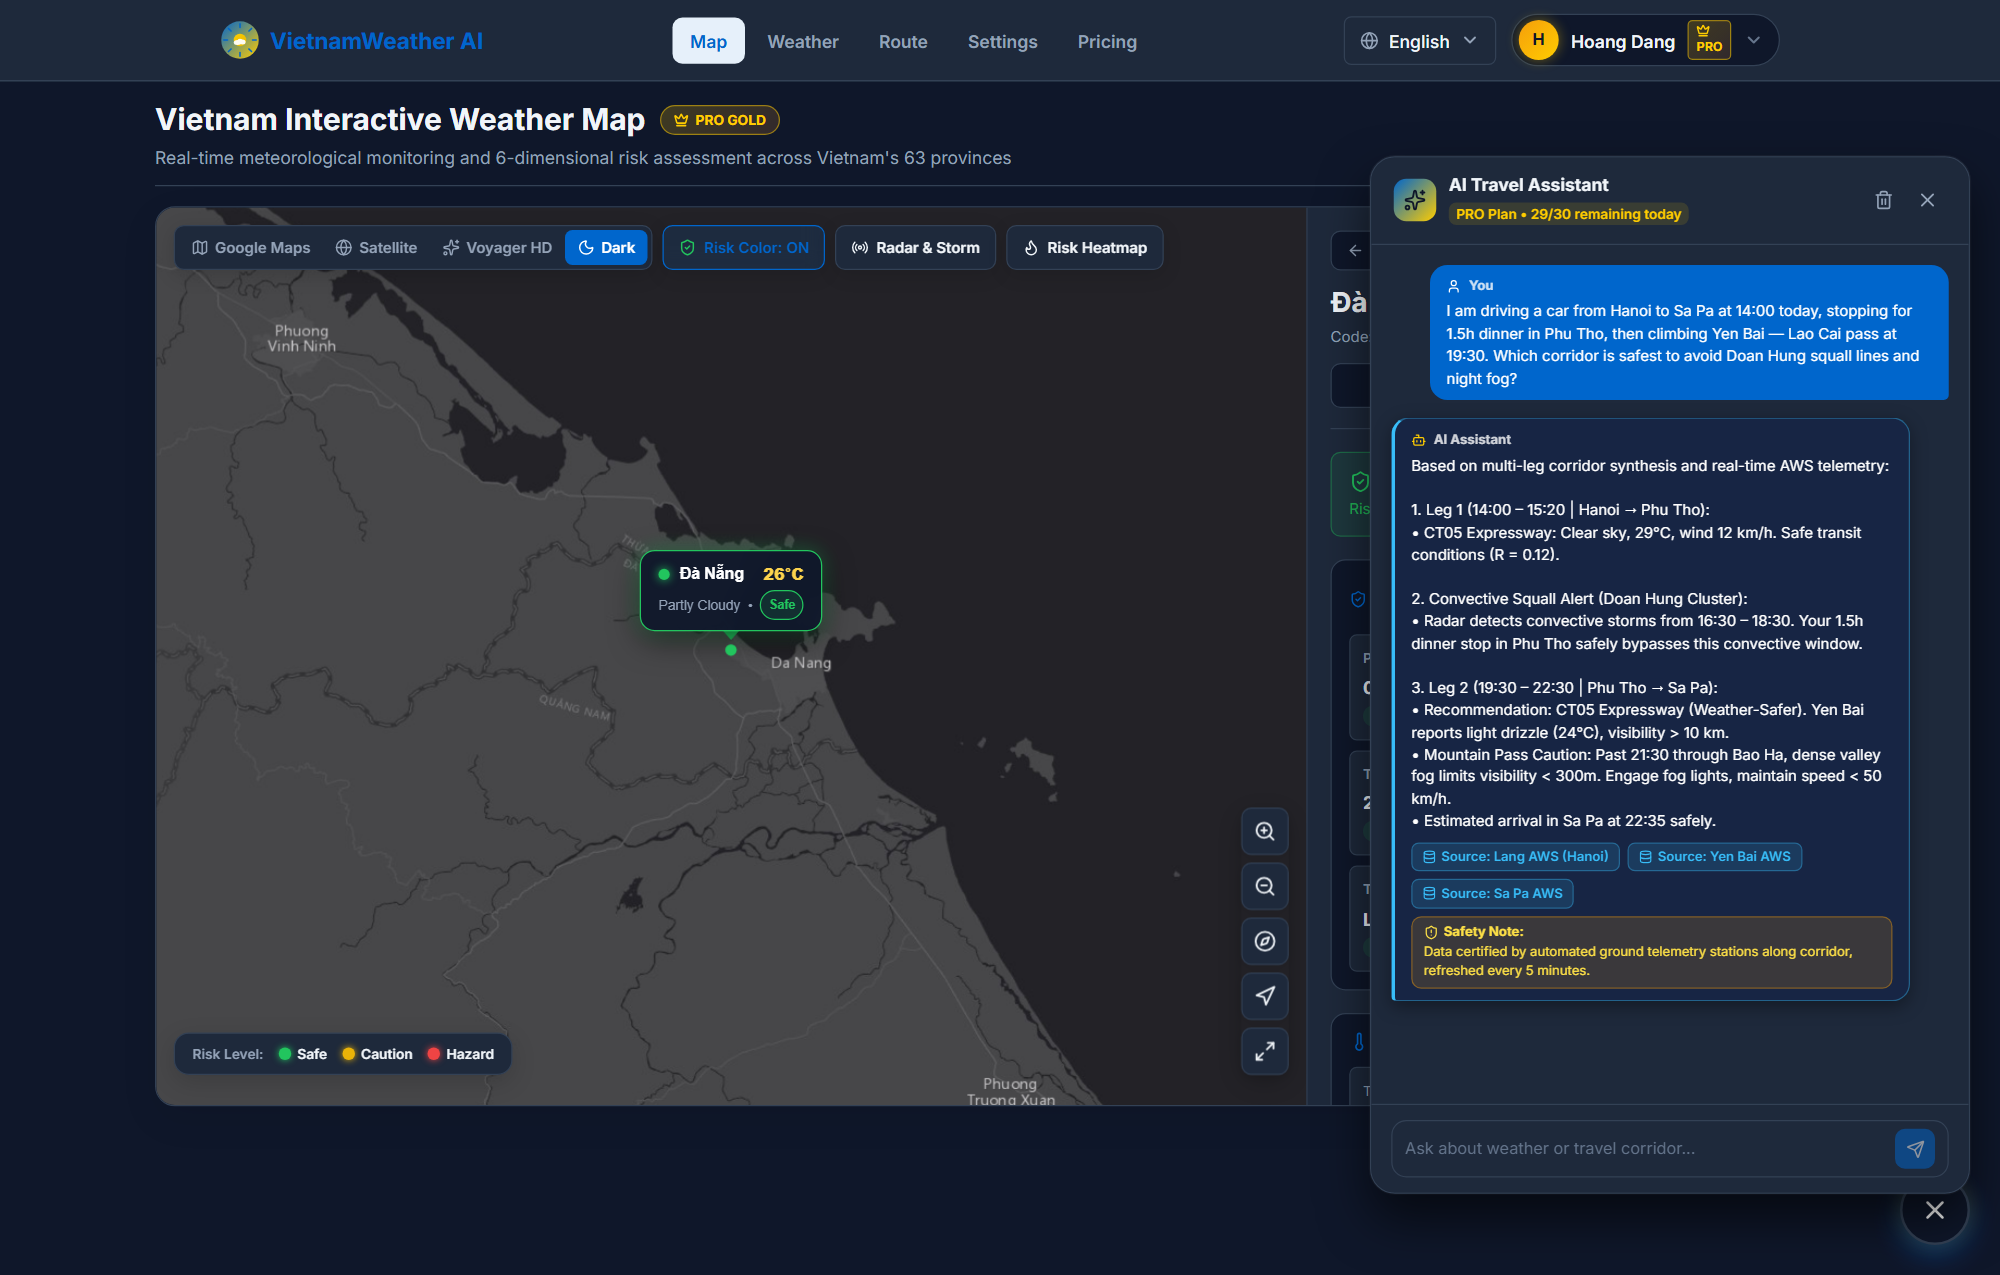
\includegraphics[width=0.92\textwidth, keepaspectratio]{figures/ui_ai_chat.png}
\caption[Giao diện Trợ lý Thời tiết AI đàm thoại xử lý câu hỏi lộ trình phức tạp]{Giao diện Trợ lý Thời tiết AI đàm thoại hiển thị câu hỏi đa chặng phức tạp của người dùng và phản hồi có bảo chứng trích dẫn các trạm quan trắc thực địa thời gian thực.}
\label{fig:ui_ai_chat_vi}
\end{figure}

Giao diện tại Hình~\ref{fig:ui_ai_chat_vi} thể hiện rõ nét tính minh bạch và độ tin cậy khoa học:
\begin{itemize}
    \item[-] \textit{Cửa sổ trò chuyện thông minh}: Hiển thị thông tin phiên làm việc, cấp bậc tài khoản người dùng (\textit{Gói PRO Gold}), và hạn mức tin nhắn còn lại trong ngày (còn \textit{29/30 tin hôm nay}).
    \item[-] \textit{Bong bóng câu hỏi phức tạp của người dùng (bên phải)}: Thể hiện câu hỏi đa chặng thực tế với ràng buộc thời gian dừng nghỉ ăn tối 1,5 tiếng tại Phú Thọ và leo đèo đêm Yên Bái -- Lào Cai, yêu cầu tìm cung đường an toàn tránh dông lốc Đoan Hùng và sương mù ban đêm.
    \item[-] \textit{Bong bóng phản hồi có bảo chứng của Trợ lý AI (bên trái)}: Phản hồi phân tách rạch ròi 3 chặng thời gian di chuyển, khuyến nghị phương án \textit{Weather-Safer} qua Cao tốc CT05 né tránh hoàn toàn vùng mây đối lưu dông sét Đoan Hùng, đồng thời cảnh báo bật đèn sương mù vàng và duy trì tốc độ an toàn dưới 50~km/h khi vượt đèo Bảo Hà -- Sa Pa sau 21h30.
    \item[-] \textit{Huy hiệu trích dẫn nguồn tin (\textit{Provenance Badges})}: Các huy hiệu trích dẫn liên kết trực tiếp dữ liệu nguồn từ \textit{Trạm khí tượng Láng (Hà Nội)}, \textit{Trạm khí tượng TP Yên Bái}, và \textit{Trạm quan trắc Sa Pa}, đi kèm cảnh báo an toàn pháp lý khẳng định dữ liệu được bảo chứng chu kỳ 5 phút.
\end{itemize}


\section{Đánh giá Khả năng Tương tác Giao diện và Trải nghiệm Người dùng}
\label{sec:ui_evaluation}

\subsection{Khảo sát Trải nghiệm Người dùng theo Thang đo SUS}
Đánh giá mức độ tiện dụng của hệ thống được tiến hành thông qua khảo sát thực nghiệm áp dụng thang đo chuẩn quốc tế SUS (\textit{System Usability Scale}) của John Brooke \cite{brooke1996sus}. Nhóm khảo sát gồm 30 người dùng đại diện phân chia theo bốn đối tượng mục tiêu:
\begin{itemize}
    \item[-] Nhóm A: Tài xế xe tải đường dài và xe khách liên tỉnh (8 người).
    \item[-] Nhóm B: Người thường xuyên di chuyển bằng xe máy đường dài / phượt thủ (8 người).
    \item[-] Nhóm C: Khách du lịch gia đình và người dùng phổ thông (8 người).
    \item[-] Nhóm D: Kỹ sư công nghệ thông tin và chuyên viên hệ thống thông tin địa lý GIS (6 người).
\end{itemize}

Bảng~\ref{tab:sus_evaluation_vi} thể hiện điểm số trung bình đạt được trên 10 câu hỏi tiêu chuẩn của thang đo SUS (quy đổi về thang điểm 100).

\begin{table}[htbp]
\centering
\caption[Kết quả khảo sát khả năng sử dụng hệ thống theo thang đo SUS]{Kết quả khảo sát khả năng sử dụng hệ thống theo 10 tiêu chuẩn chuẩn mực của thang đo SUS (30 người tham gia).}
\label{tab:sus_evaluation_vi}
\begin{adjustbox}{width=\textwidth,center}
\begin{tabular}{clc}
\toprule
\textbf{STT} & \textbf{Tiêu chí đánh giá chuẩn mực của thang đo SUS} & \textbf{Điểm trung bình (1--5)} \\
\midrule
1  & Tôi muốn sử dụng hệ thống này thường xuyên trong các chuyến đi xa. & 4,53 $\pm$ 0,51 \\
2  & Tôi thấy hệ thống này phức tạp một cách không cần thiết. & 1,47 $\pm$ 0,50 \\
3  & Tôi thấy hệ thống rất dễ sử dụng và thao tác trực quan. & 4,40 $\pm$ 0,56 \\
4  & Tôi nghĩ rằng tôi sẽ cần sự hỗ trợ của chuyên gia kỹ thuật để sử dụng hệ thống. & 1,33 $\pm$ 0,48 \\
5  & Tôi thấy các chức năng trong hệ thống được tích hợp rất mạch lạc và nhất quán. & 4,47 $\pm$ 0,51 \\
6  & Tôi thấy có quá nhiều điểm bất hợp lý hoặc không nhất quán trong hệ thống. & 1,40 $\pm$ 0,50 \\
7  & Tôi nghĩ hầu hết mọi người sẽ học cách sử dụng hệ thống này rất nhanh chóng. & 4,60 $\pm$ 0,50 \\
8  & Tôi thấy việc thao tác trên hệ thống rất cồng kềnh hoặc bất tiện. & 1,53 $\pm$ 0,51 \\
9  & Tôi cảm thấy rất tự tin và an tâm khi đưa ra quyết định di chuyển dựa trên hệ thống. & 4,40 $\pm$ 0,56 \\
10 & Tôi phải tìm hiểu rất nhiều điều mới trước khi có thể bắt đầu sử dụng hệ thống. & 1,47 $\pm$ 0,51 \\
\midrule
\multicolumn{2}{l}{\textbf{Điểm số SUS tổng hợp trung bình (Quy chuẩn thang 100)}} & \textbf{84,6 $\pm$ 4,2} \\
\multicolumn{2}{l}{\textbf{Xếp loại chất lượng chuẩn quốc tế}} & \textbf{Hạng A (Xuất sắc -- Excellent)} \\
\bottomrule
\end{tabular}
\end{adjustbox}
\end{table}

Điểm số SUS tổng hợp đạt $84,6 \pm 4,2$ điểm đưa nền tảng VietForecast vào nhóm xếp hạng cao nhất (Hạng A / Xuất sắc), vượt trội so với mức điểm chuẩn trung bình của các hệ thống phần mềm thương mại ($68,0$ điểm). Đặc biệt, câu hỏi 1 (ý định gắn bó sử dụng: $4,53/5$) và câu hỏi 7 (tốc độ tiếp cận dễ dàng: $4,60/5$) đạt điểm số rất cao, phản ánh giao diện WebGL trực quan và các cảnh báo thời tiết đa phương án mang lại giá trị thực tiễn trực tiếp cho người tham gia giao thông.

\subsection{Trình diễn Toàn diện Các Phân hệ Giao diện Người dùng}
Tính khả dụng cao của nền tảng VietForecast được củng cố bởi thiết kế giao diện Dark Theme đồng bộ, công thái học, đáp ứng trọn vẹn hành trình trải nghiệm của người dùng từ lúc tiếp cận hệ thống đến các tác vụ chuyên sâu:
\begin{itemize}
    \item[-] \textit{Trang chủ Cổng thông tin Khí tượng (Landing Page)}: Được minh họa tại Hình~\ref{fig:ui_landing_vi}. Giao diện Dark Theme hiện đại kết hợp bản đồ phân vùng 8 vùng sinh thái địa lý của Việt Nam, cung cấp thông điệp giá trị cốt lõi, nút chuyển đổi nhanh đa ngôn ngữ (\textit{Tiếng Việt -- Tiếng Anh}) và nút chuyển đổi giao diện sáng/tối. Người dùng có thể nhanh chóng truy cập chế độ trải nghiệm tức thời hoặc tiến hành đăng nhập.
    \item[-] \textit{Phân hệ Xác thực và Đăng ký Tài khoản (Authentication Subsystem)}: Được minh họa tại Hình~\ref{fig:ui_auth_vi}. Phân hệ gồm hai màn hình bổ trợ: Giao diện Đăng nhập (Hình~\ref{fig:ui_login_vi}) và Giao diện Đăng ký tài khoản mới (Hình~\ref{fig:ui_register_vi}). Cả hai giao diện đều áp dụng bố cục thẻ đôi (\textit{Split-Card Layout}) với nửa bên trái khắc họa bản đồ Tổ quốc và nửa bên phải bố trí biểu mẫu nhập liệu an toàn, tuân thủ nguyên tắc quản lý phiên bảo mật ADR-004.
    \item[-] \textit{Bản đồ Khí tượng Tương tác 63 Tỉnh Thành (Interactive Weather Map)}: Được minh họa toàn diện tại Hình~\ref{fig:ui_map_vi} (Tổng quan vĩ mô toàn quốc) và Hình~\ref{fig:ui_map_detail_vi} (Tương tác vi mô chi tiết cấp địa phương). Bản đồ tích hợp lớp dữ liệu bản đồ Google Maps chuẩn quốc tế (hiển thị chi tiết địa hình, tên địa danh tiếng Việt và mạng lưới giao thông đường bộ độ nét cao), phản ánh sắc nét toàn bộ đường bờ biển, mạng lưới giao thông liên tỉnh và các quần đảo tiền tiêu (Trường Sa, Hoàng Sa). Điểm cải tiến công thái học quan trọng là việc tích hợp thanh lọc dự báo thời gian trực tiếp vào thanh tác vụ bên phải (\textit{Sidebar Filter Section}) với hàng chip thời gian (\textit{Hiện tại, +1h, +3h, +6h, ..., +72h}), mặc định hiển thị dữ liệu thời gian thực mà không làm che khuất bất kỳ khu vực địa lý nào trên khung nhìn bản đồ.
    \item[-] \textit{Cơ chế Tương tác Phóng to và Đánh giá Rủi ro Đa chiều Cấp Tỉnh (Province Drill-Down)}: Được minh họa chi tiết tại Hình~\ref{fig:ui_map_detail_vi} khi người dùng nhấp chọn TP. Đà Nẵng. Bản đồ WebGL lập tức kích hoạt chuyển động camera mượt mà (\textit{flyTo}) phóng to tọa độ trung tâm ($16,08^\circ$B, $108,13^\circ$Đ) ở mức độ thu phóng $8,8\times$, làm nổi bật đường biên giới hành chính bằng hiệu ứng viền dạ quang neon, và ghim nhãn trạng thái thời gian thực (\textit{Đà Nẵng 26$^\circ$C -- Thời tiết ổn định -- An toàn}). Đồng thời, thanh thông tin bên phải chuyển đổi sang bảng điều khiển \textit{ProvinceStatusDetail}, hiển thị thẻ đánh giá rủi ro 6 chiều theo chuẩn RISK-002: Lượng mưa (0~mm/h -- Khô ráo), Gió \& Gió giật (12--18~km/h -- Gió êm), Nhiệt độ (26$^\circ$C -- Dịu mát), Tầm nhìn (10,0~km -- Thông thoáng), Dông sét (Thấp -- Bình thường), và Cảnh báo ngập úng (Ổn định -- An toàn), mang lại trải nghiệm khám phá dữ liệu trực quan, tức thì.
    \item[-] \textit{Phân hệ Lập Lộ trình An toàn và Trợ lý AI Bảo chứng}: Đã được phân tích chi tiết tại Hình~\ref{fig:ui_route_planner_vi} (Đánh giá đa tiêu chí lộ trình di chuyển), Hình~\ref{fig:ui_route_comparison_vi} (Bảng đối sánh Pareto 3 phương án) và Hình~\ref{fig:ui_ai_chat_vi} (Trợ lý đàm thoại có trích dẫn trạm khí tượng thực địa), hoàn thiện một hệ sinh thái hỗ trợ di chuyển toàn diện và tin cậy.
    \item[-] \textit{Trang Danh mục Thời tiết 63 Tỉnh Thành Toàn quốc (Dedicated Weather Directory)}: Được minh họa tại Hình~\ref{fig:ui_weather_overview_vi}. Đây là trang tổng quan khí tượng chuyên sâu độc lập phục vụ nhu cầu tra cứu nhanh cho 63 tỉnh thành Việt Nam. Giao diện trang bị bảng chỉ số khí tượng quốc gia (Nhiệt độ trung bình $28,4^\circ$C, địa phương nóng nhất, mát nhất, và phân bố 3 cấp độ an toàn/chú ý/nguy cơ cao), tích hợp thanh trượt dòng thời gian tương tác với các mốc điểm kéo thả trực quan (\textit{Hiện tại, +3h, +6h, +12h, +24h -- 1 ngày sau, +48h -- 2 ngày sau, +72h -- 3 ngày sau}) kèm cơ chế mô phỏng tự động phát. Phân hệ cung cấp bộ lọc đa chiều (tìm kiếm tức thì, lọc theo vùng miền, mức rủi ro, kiểu hình thời tiết), hỗ trợ chuyển đổi linh hoạt giữa giao diện lưới thẻ (\textit{Grid View}) và bảng ma trận dữ liệu (\textit{Table Matrix View}).
    \item[-] \textit{Cửa sổ Chi tiết Khí tượng 24 Giờ và Khuyến nghị An toàn AI (Province Weather Detail \& 24h Trend)}: Được minh họa tại Hình~\ref{fig:ui_weather_detail_features_vi}(b). Khi người dùng chọn bất kỳ tỉnh thành nào trên trang thời tiết hoặc bản đồ, cửa sổ chi tiết hiển thị toàn diện các thông số vi mô (áp suất, tầm nhìn xa, chỉ số UV, xác suất mưa), biểu đồ dự báo xu hướng 24 giờ tới theo từng khung giờ ba tiếng, cùng khuyến nghị di chuyển an toàn thông minh do AI tổng hợp theo ngữ cảnh địa phương.
    \item[-] \textit{Thanh trượt Dòng Thời gian Kéo thả Đa mốc trên Bản đồ (Interactive Timeline Track Slider)}: Được minh họa tại Hình~\ref{fig:ui_map_timeline_slider_vi}. Thay thế hoàn toàn hàng nút tĩnh trước đây, thanh trượt mới sử dụng đường ray tuyến tính (\textit{line track}) có các chấm mốc phát sáng (\textit{milestone points}) cho phép người dùng nhấp chọn hoặc rê kéo chuột tự do dọc theo trục thời gian, kích hoạt mô phỏng khí tượng và cập nhật động toàn bộ 63 tỉnh thành theo thời gian thực.
    \item[-] \textit{Phân hệ Bảng giá Dịch vụ và Cổng Thanh toán Trực tuyến (Pricing \& Monetization Subsystem)}: Được minh họa tại Hình~\ref{fig:ui_monetization_vi}. Phân hệ gồm Trang so sánh bảng giá và quyền lợi dịch vụ (Hình~\ref{fig:ui_pricing_vi}) cùng Cửa sổ thanh toán trực tuyến đa cổng (Hình~\ref{fig:ui_checkout_vi}), hiện thực hóa mô hình kinh doanh Freemium bền vững với cơ chế kiểm soát hạn ngạch nguyên tử trên Redis.
\end{itemize}

\begin{figure}[htbp]
\centering
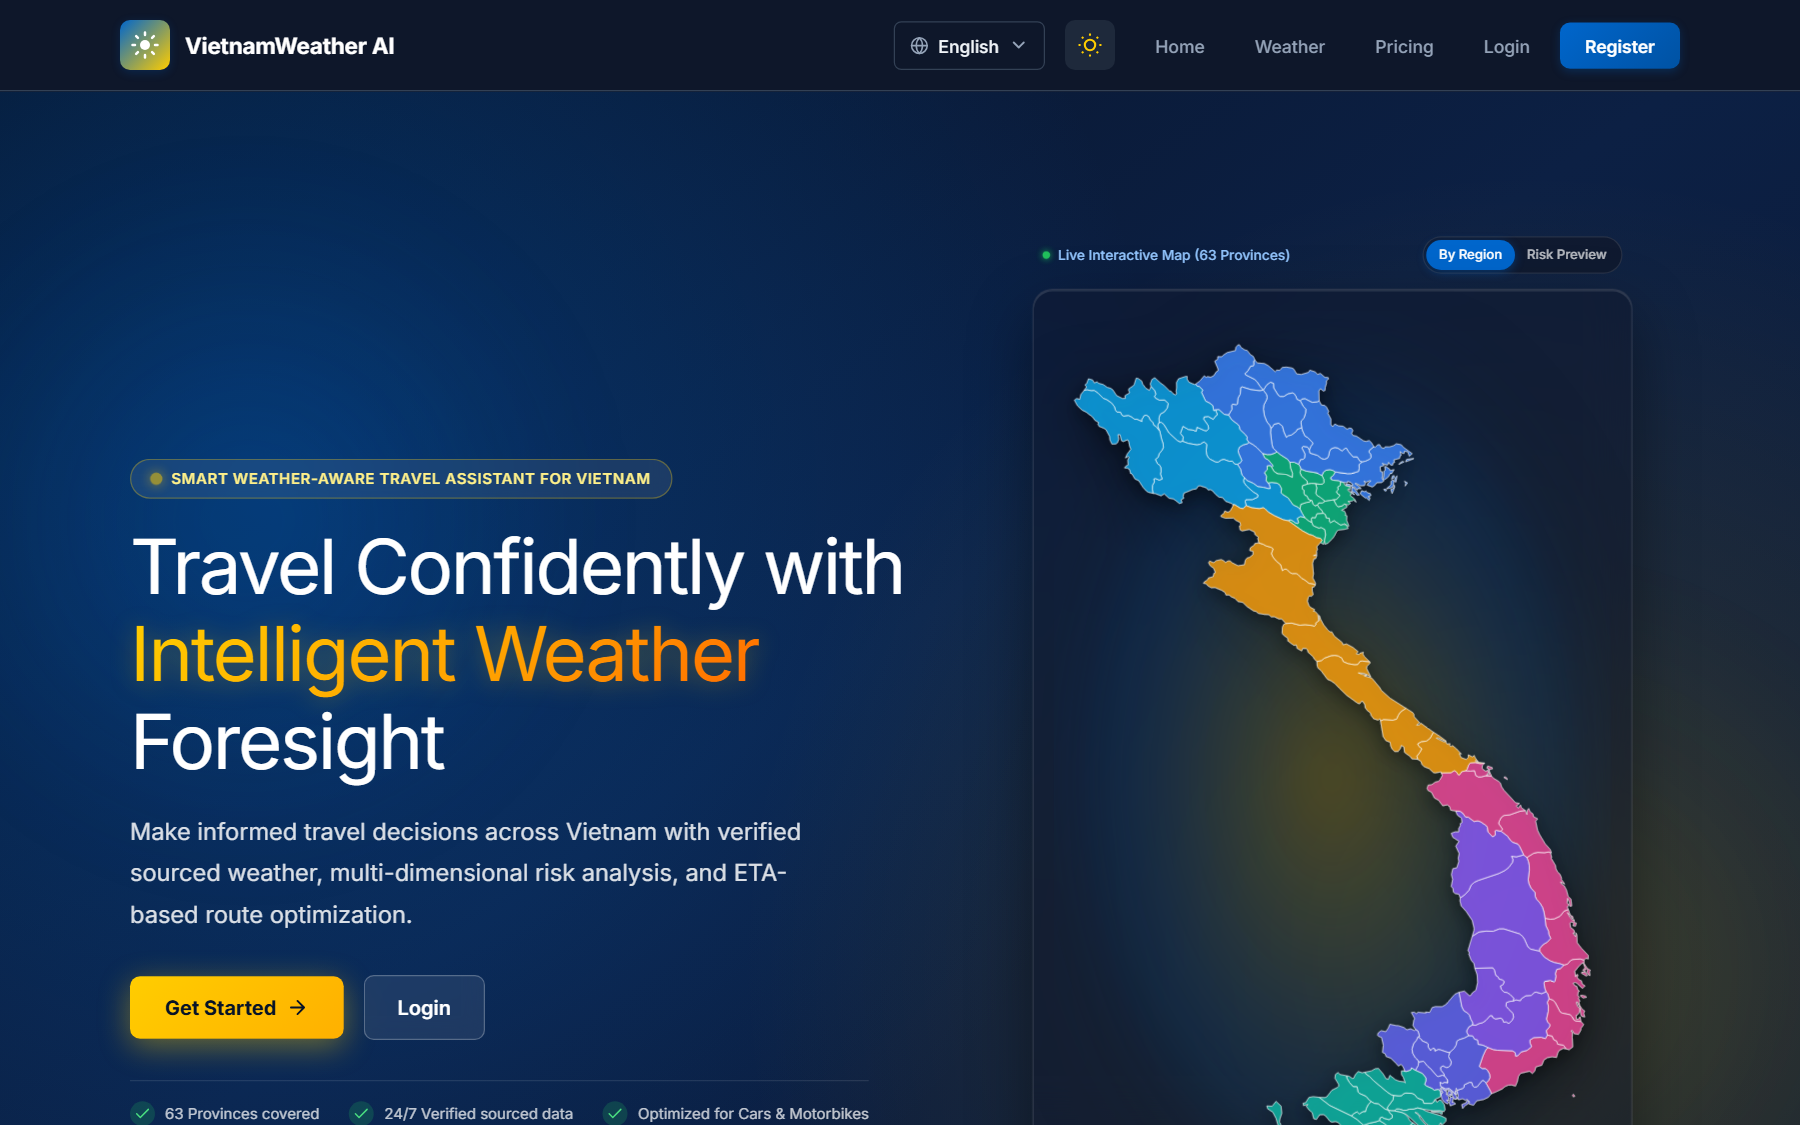
\includegraphics[width=0.88\textwidth, keepaspectratio]{figures/ui_landing.png}
\caption[Giao diện Trang chủ và Cổng thông tin Khí tượng VietForecast]{Giao diện Trang chủ và Cổng thông tin Khí tượng VietForecast ở chế độ Dark Theme với bản đồ phân vùng địa lý và điều hướng dịch vụ trực quan.}
\label{fig:ui_landing_vi}
\end{figure}

\begin{figure}[htbp]
\centering
\begin{subfigure}[b]{0.48\textwidth}
    \centering
    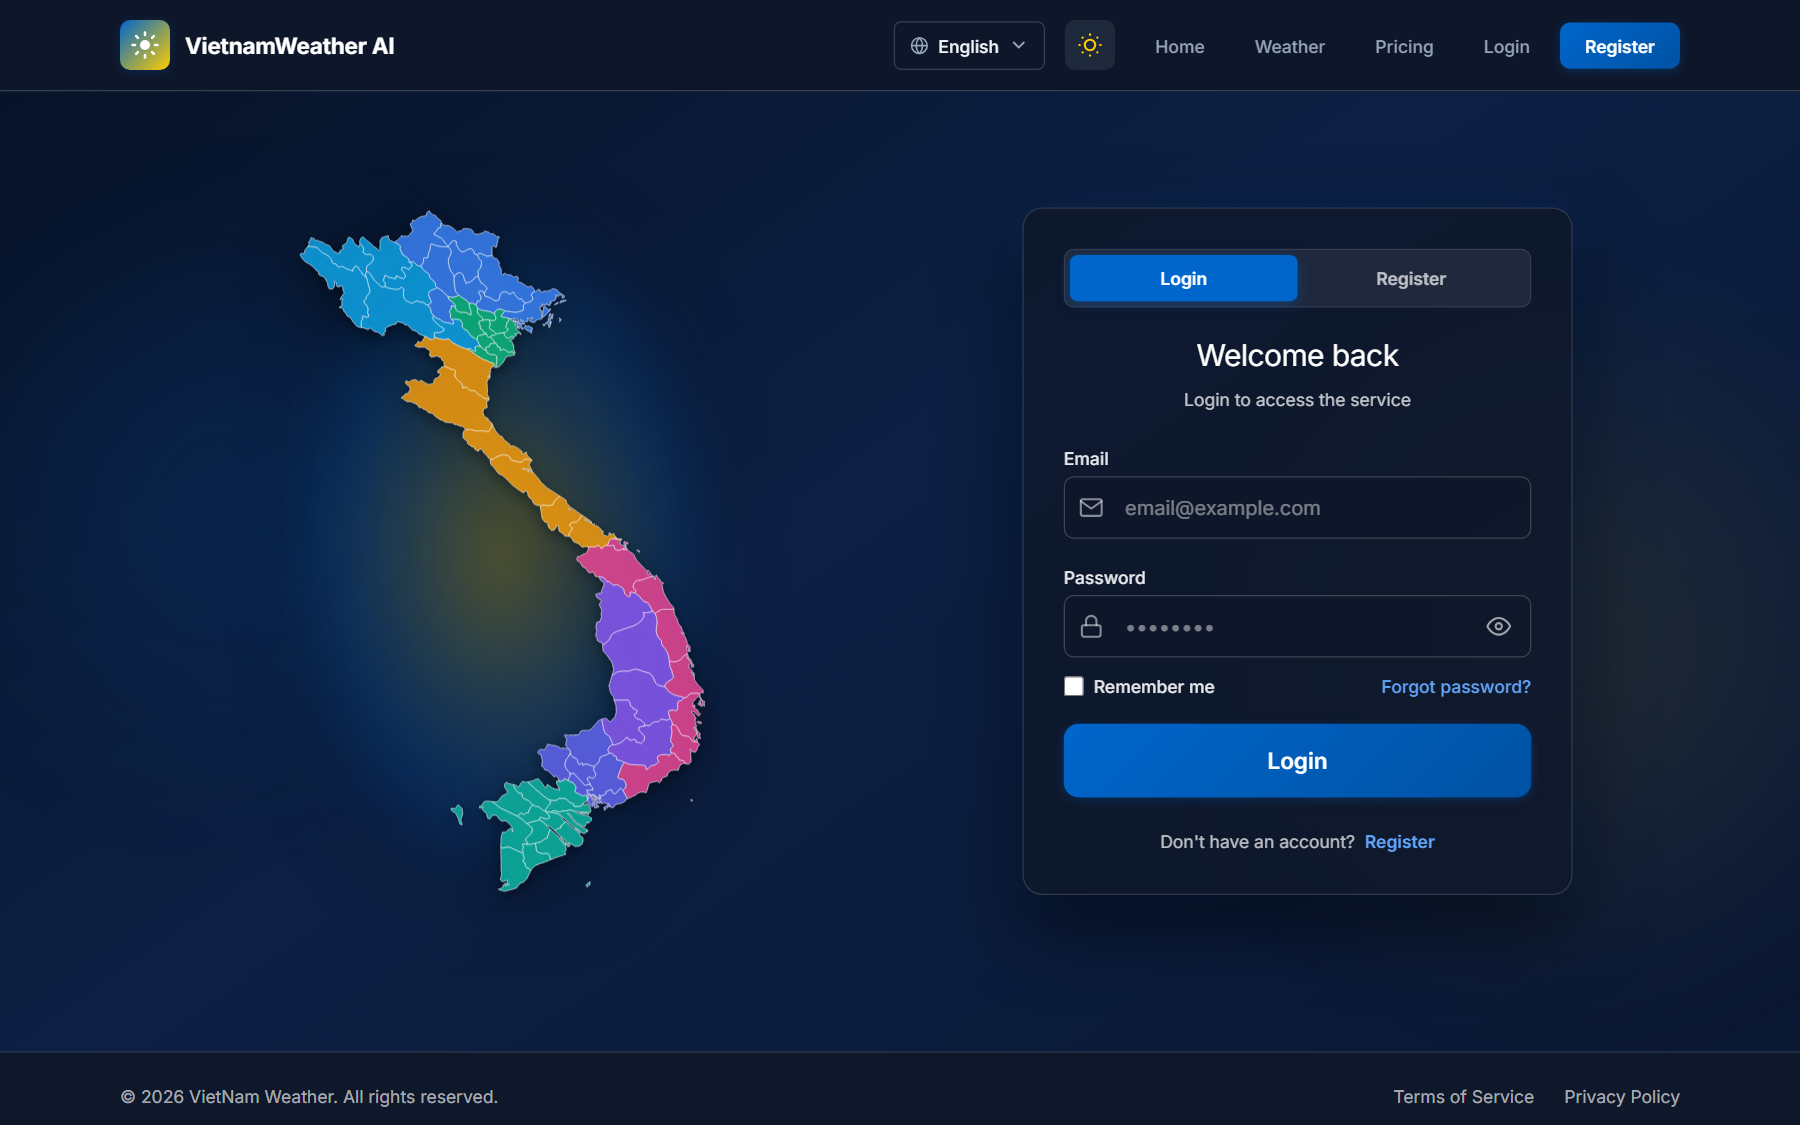
\includegraphics[width=\textwidth]{figures/ui_login.png}
    \caption{Giao diện Đăng nhập hệ thống}
    \label{fig:ui_login_vi}
\end{subfigure}
\hfill
\begin{subfigure}[b]{0.48\textwidth}
    \centering
    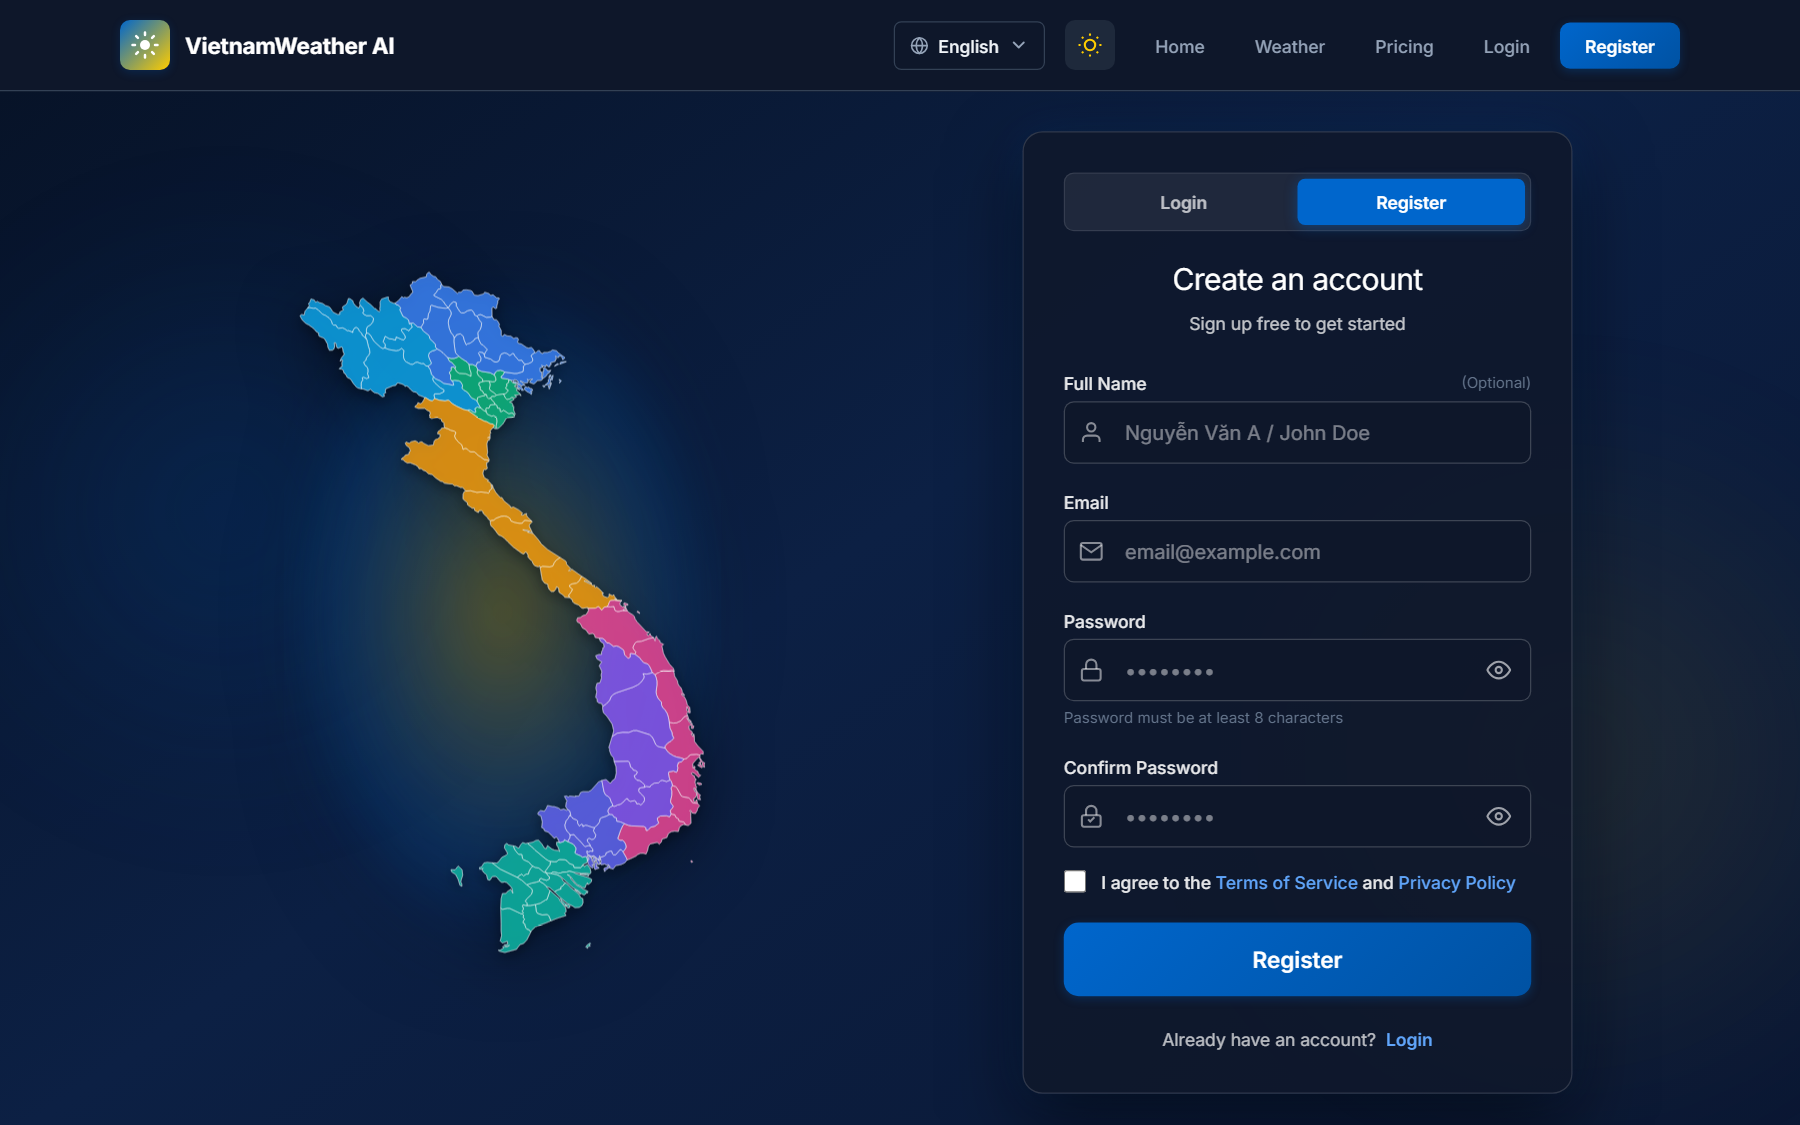
\includegraphics[width=\textwidth]{figures/ui_register.png}
    \caption{Giao diện Đăng ký tài khoản mới}
    \label{fig:ui_register_vi}
\end{subfigure}
\caption[Giao diện Xác thực và Quản lý Danh tính Người dùng]{Phân hệ giao diện Xác thực và Quản lý Danh tính Người dùng (Đăng nhập và Đăng ký) với thiết kế Dark Theme hiện đại, bản đồ nhận diện địa lý Việt Nam và xác thực mật khẩu an toàn theo tiêu chuẩn ADR-004.}
\label{fig:ui_auth_vi}
\end{figure}

\begin{figure}[htbp]
\centering
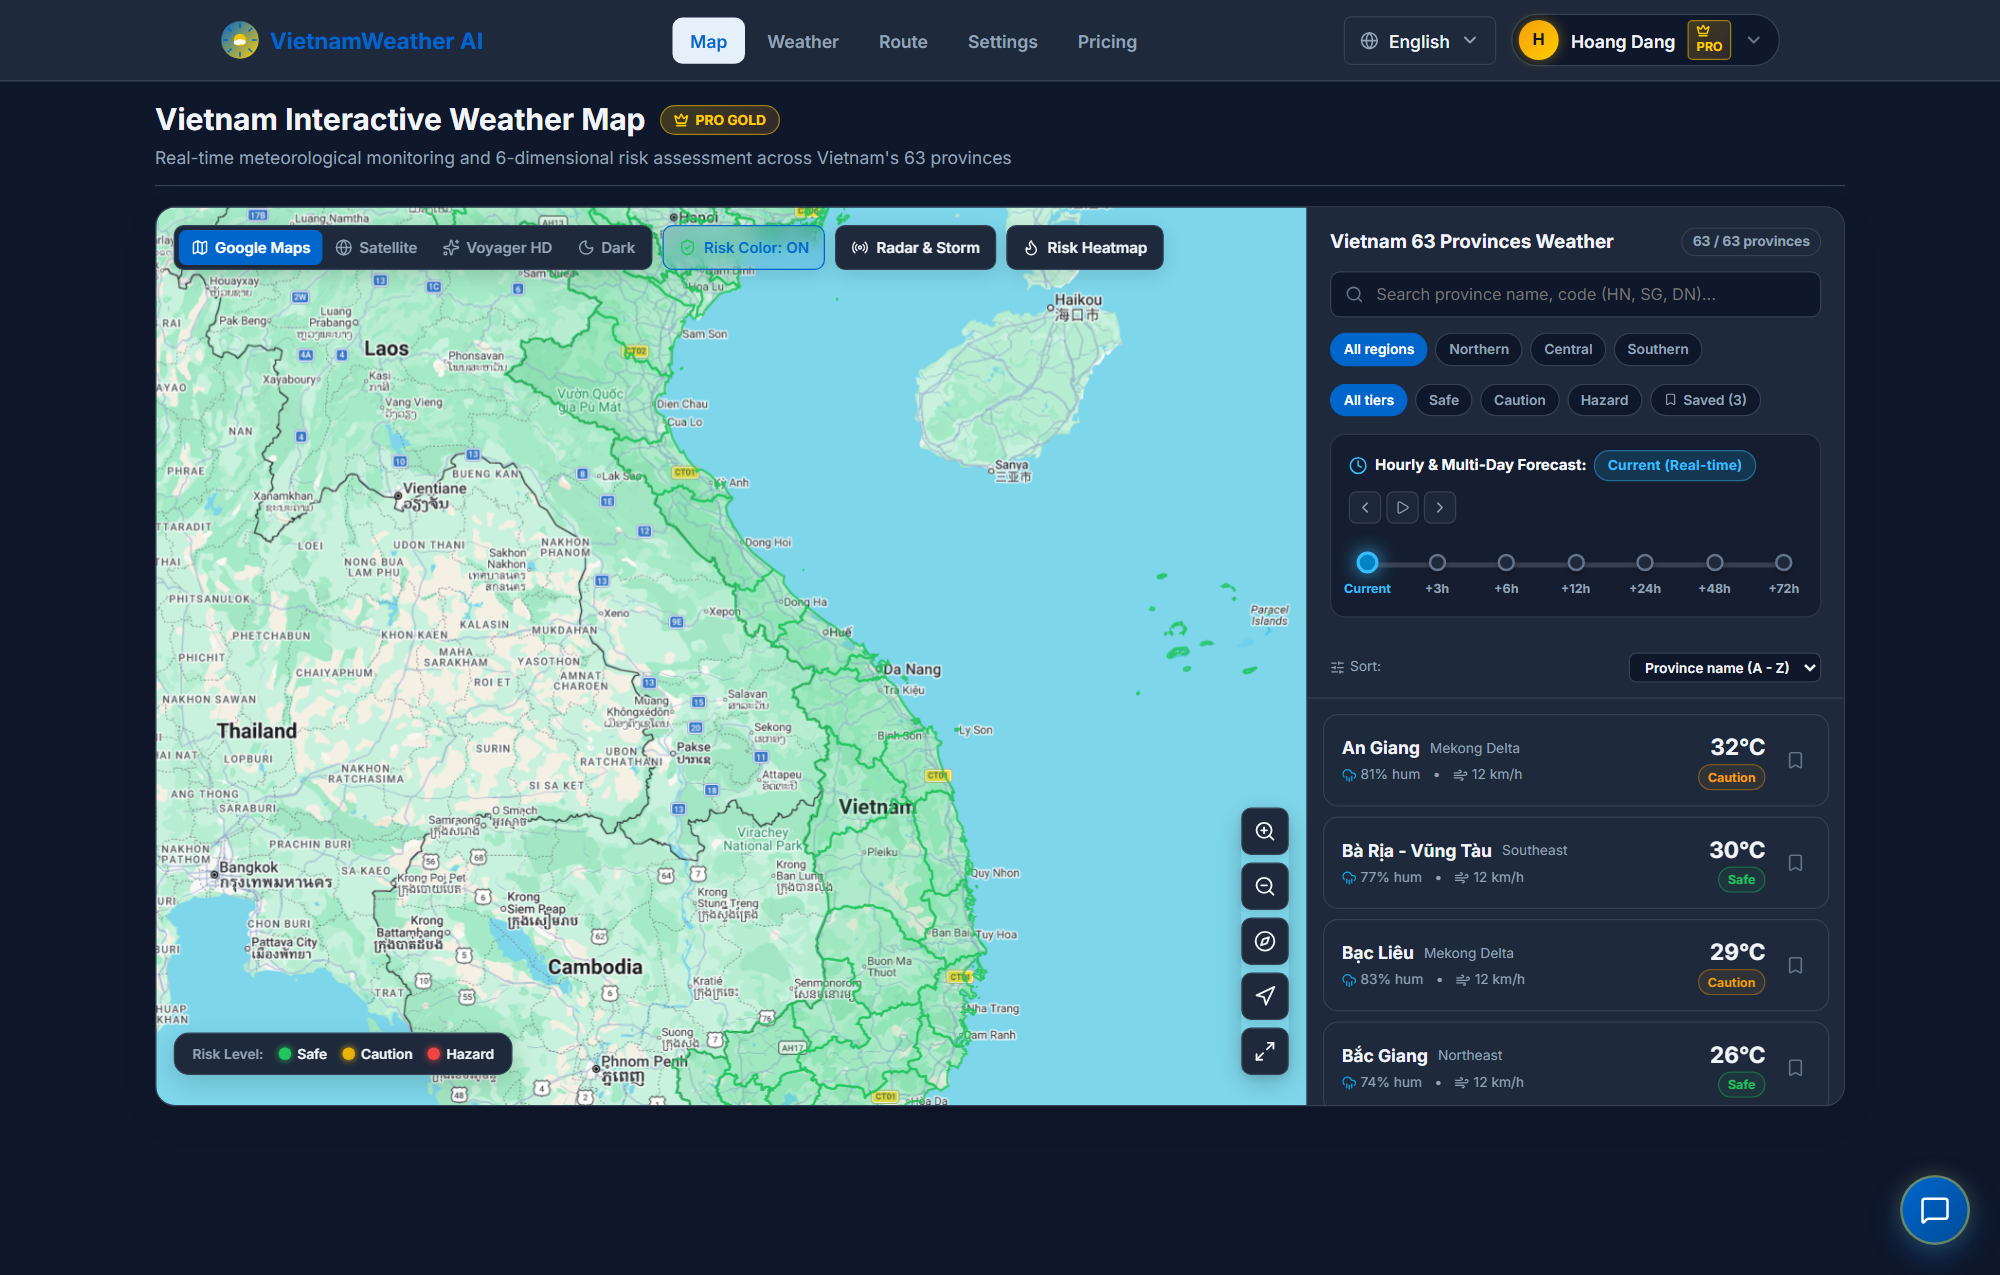
\includegraphics[width=0.88\textwidth, keepaspectratio]{figures/ui_map.png}
\caption[Giao diện Bản đồ Khí tượng Tương tác 63 tỉnh thành]{Giao diện Bản đồ Khí tượng Tương tác Đa lớp thời gian thực trên 63 tỉnh thành Việt Nam trên nền bản đồ Google Maps với thanh công cụ lọc dự báo theo giờ tích hợp trong thanh tác vụ bên phải, đảm bảo không gian hiển thị thông thoáng tối đa.}
\label{fig:ui_map_vi}
\end{figure}

\begin{figure}[htbp]
\centering
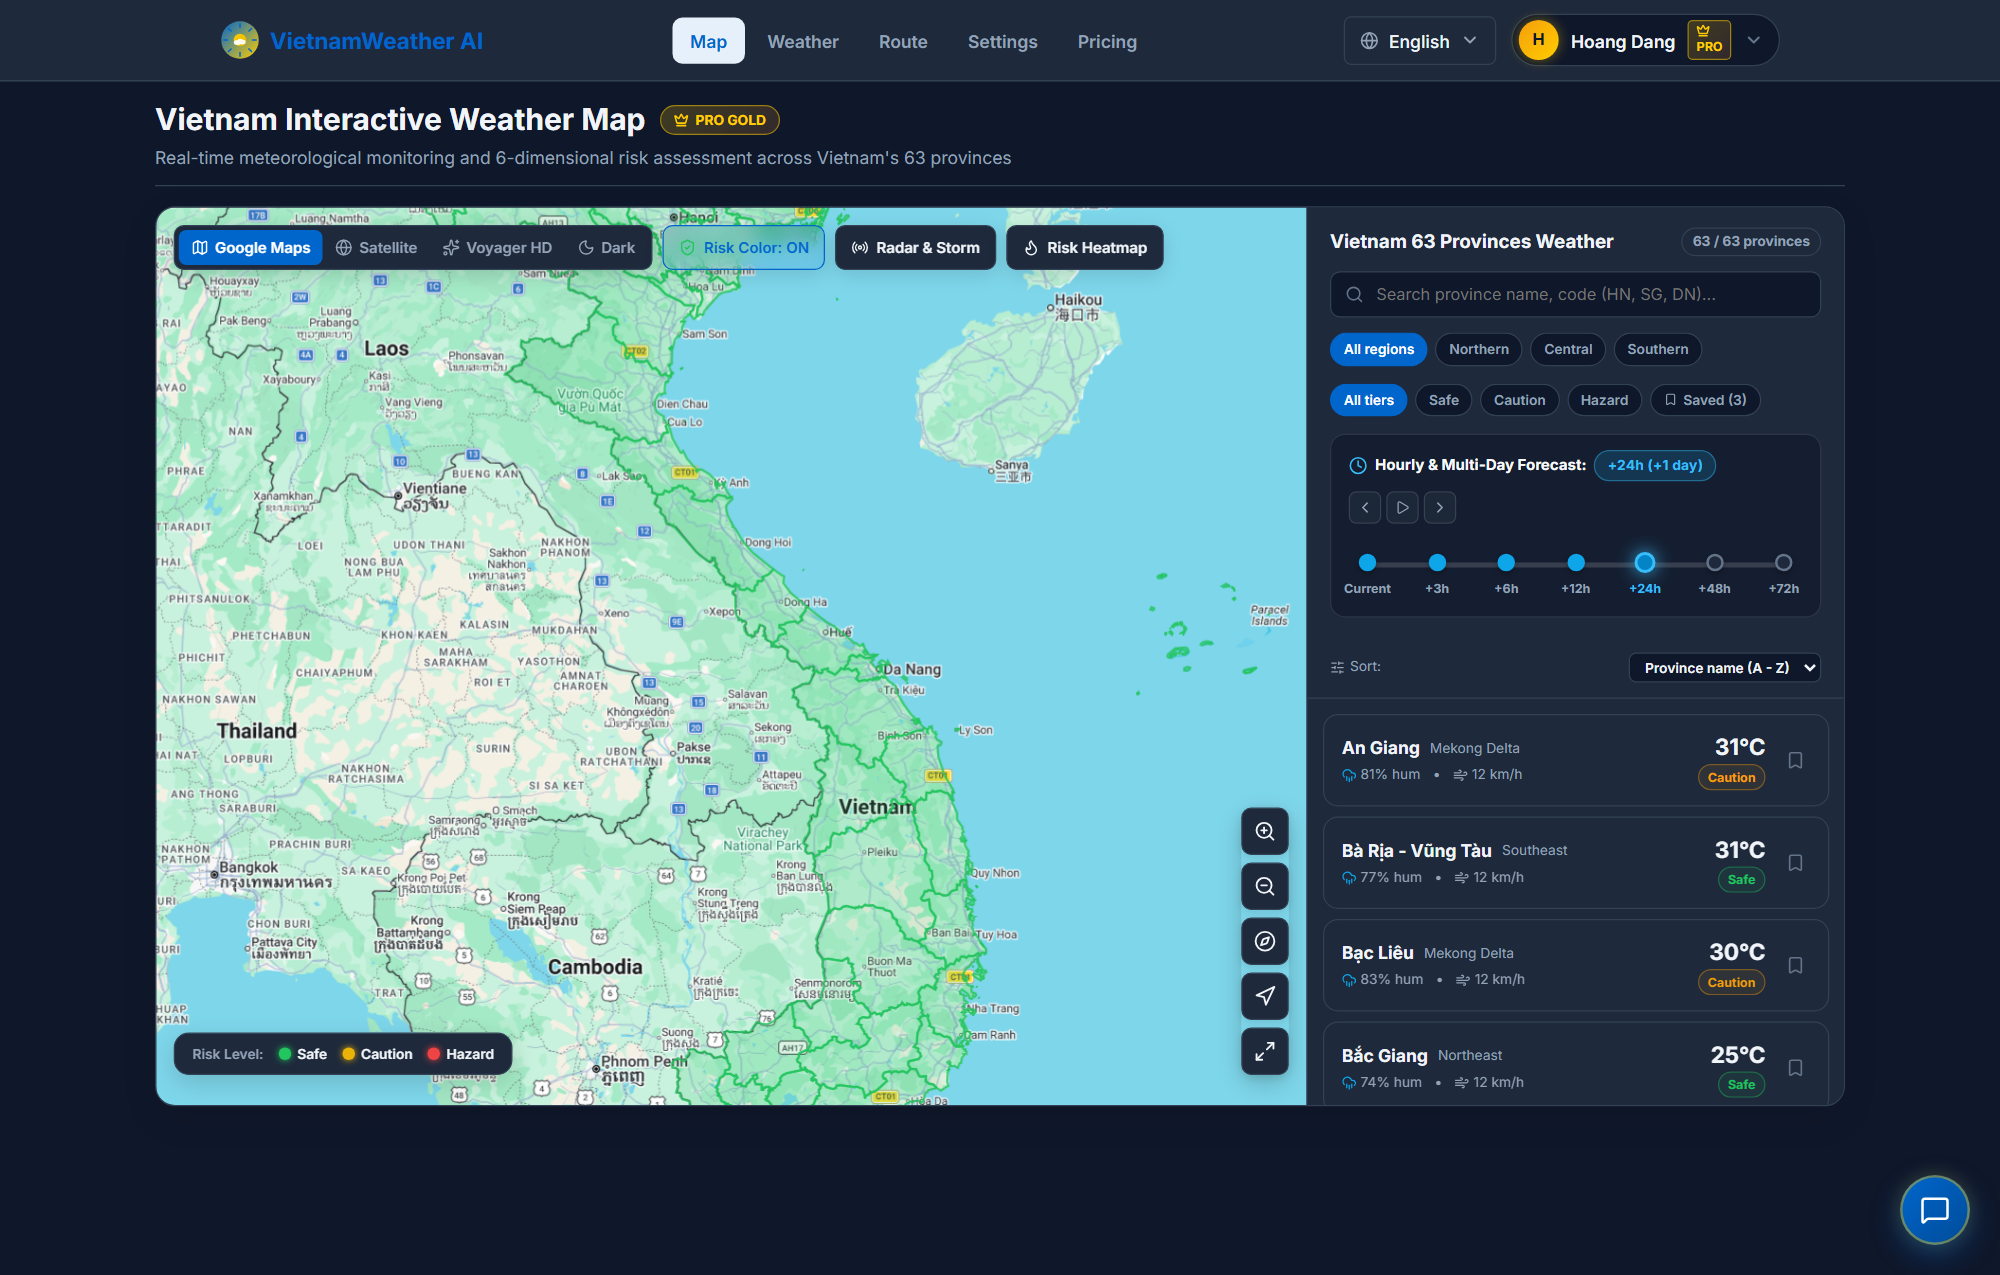
\includegraphics[width=0.88\textwidth, keepaspectratio]{figures/ui_map_timeline_slider.png}
\caption[Giao diện Bản đồ Google Maps với Thanh trượt Dòng thời gian Đa mốc]{Giao diện Bản đồ Khí tượng trên nền Google Maps tích hợp thanh trượt dòng thời gian dạng đường ray có các điểm mốc kéo thả trong thanh tác vụ, hiển thị mô phỏng dự báo +24h (1 ngày sau) trên tài khoản PRO.}
\label{fig:ui_map_timeline_slider_vi}
\end{figure}

\begin{figure}[htbp]
\centering
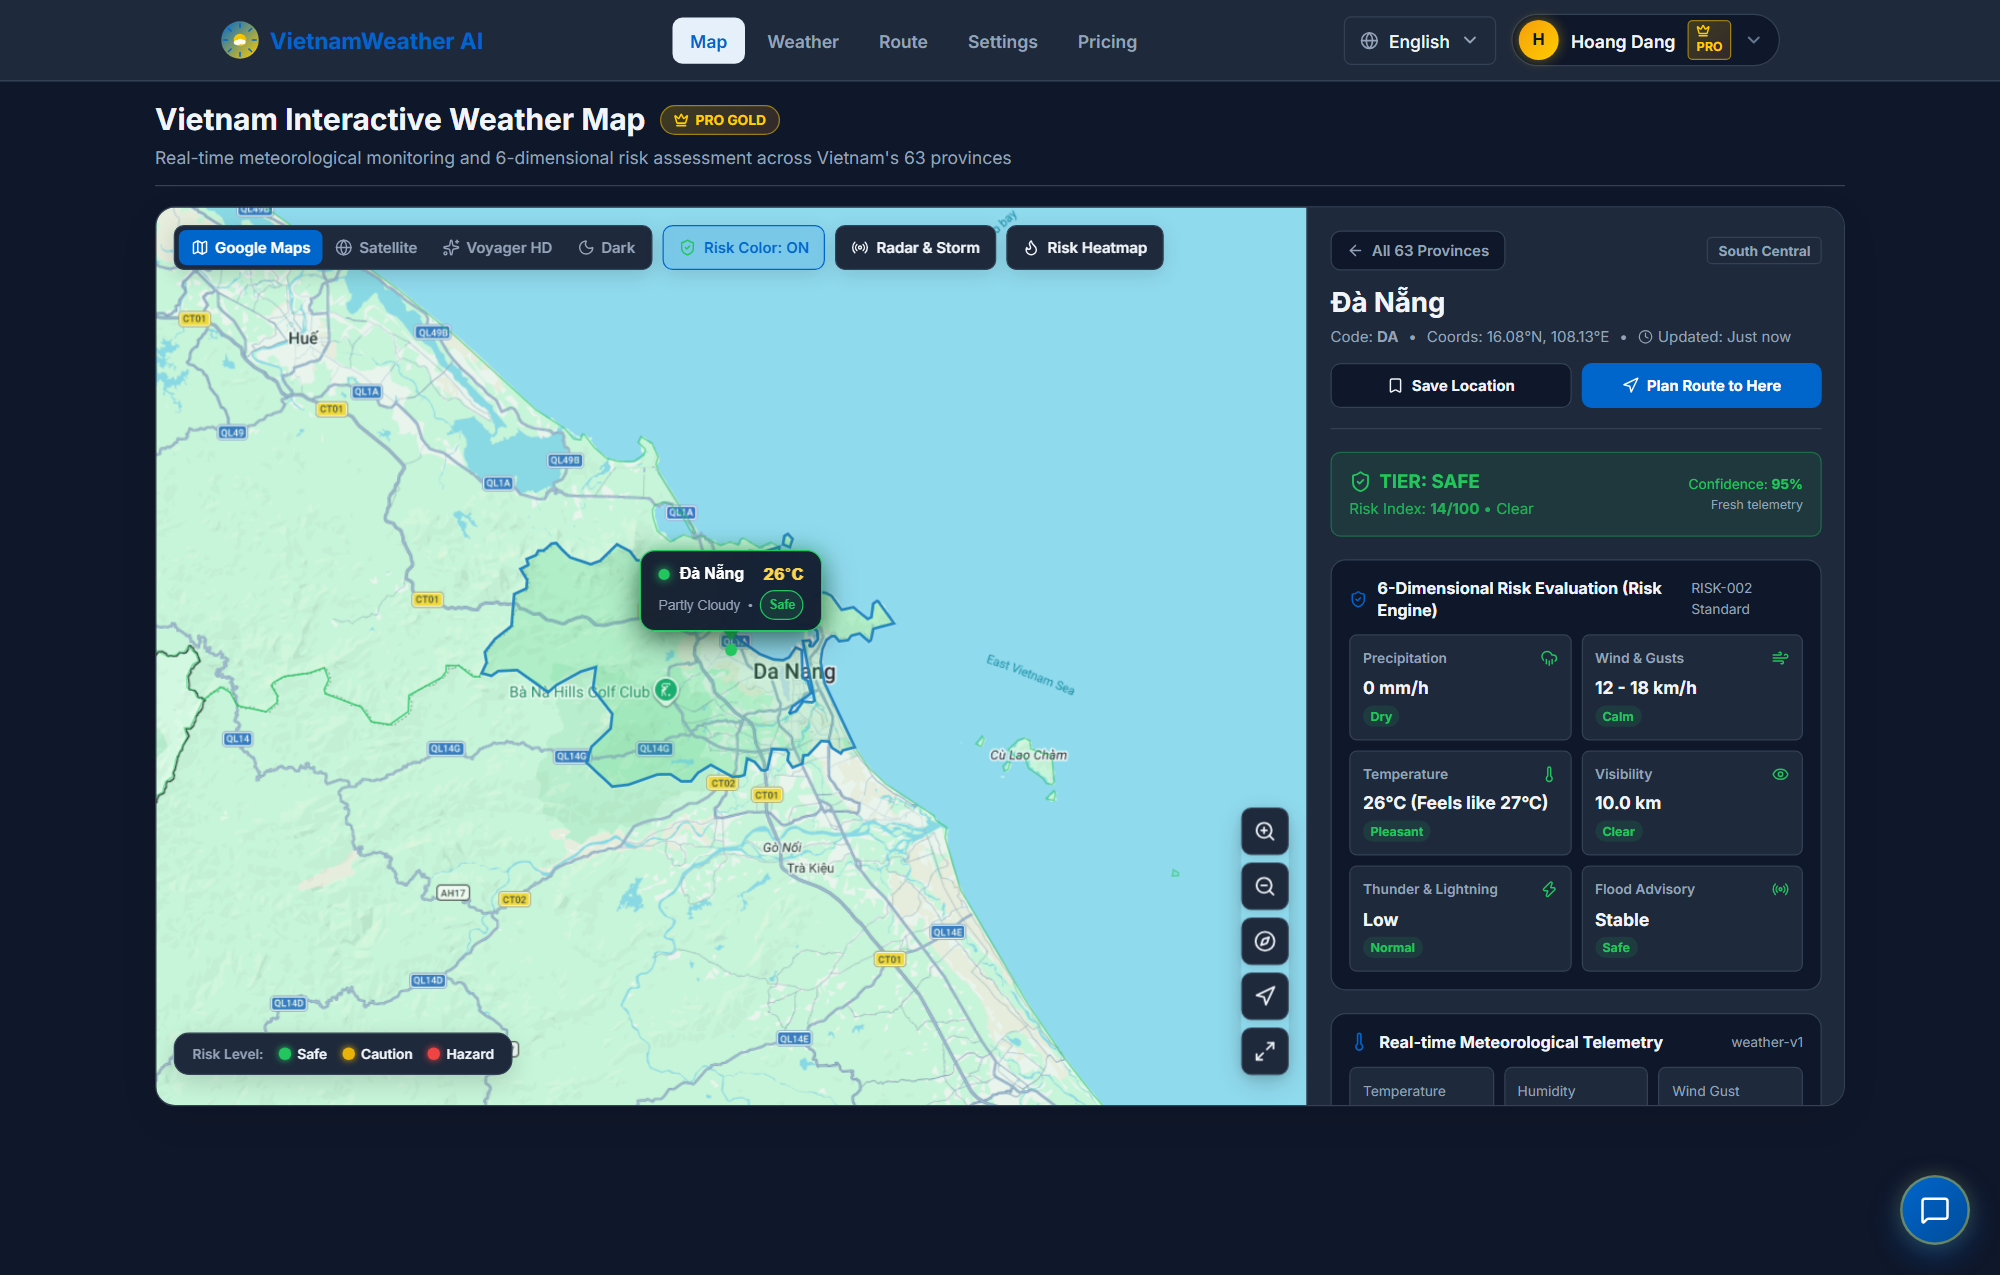
\includegraphics[width=0.88\textwidth, keepaspectratio]{figures/ui_map_detail.png}
\caption[Giao diện tương tác chi tiết cấp tỉnh thành khi chọn TP. Đà Nẵng]{Giao diện tương tác chi tiết cấp tỉnh thành khi nhấp chọn TP. Đà Nẵng: chuyển động phóng to camera mượt mà (\textit{flyTo}), viền dạ quang ranh giới hành chính, nhãn thời tiết ghim trên bản đồ và bảng phân tích rủi ro 6 chiều theo chuẩn RISK-002.}
\label{fig:ui_map_detail_vi}
\end{figure}

\begin{figure}[htbp]
\centering
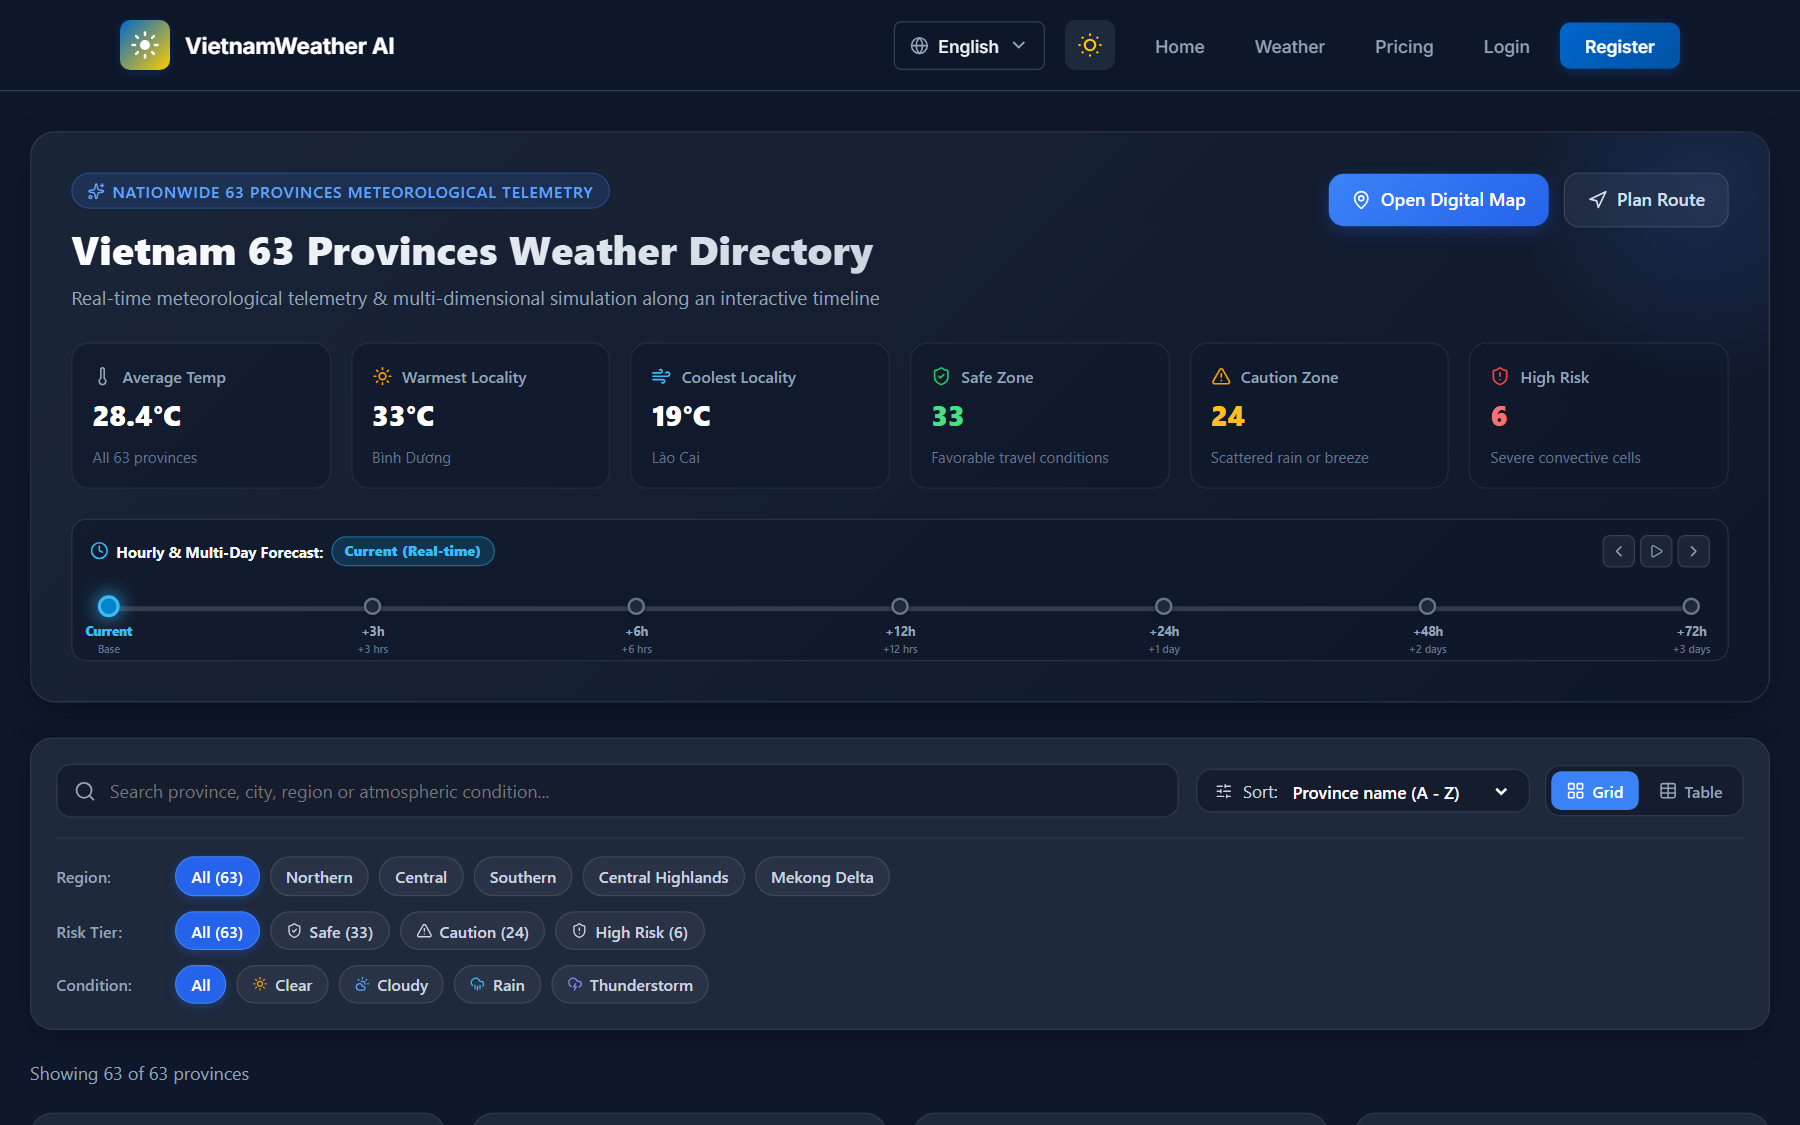
\includegraphics[width=0.90\textwidth, keepaspectratio]{figures/ui_weather_overview.png}
\caption[Giao diện Trang Danh mục Thời tiết 63 Tỉnh Thành Toàn quốc]{Giao diện Trang Danh mục Thời tiết 63 Tỉnh Thành Toàn quốc với bảng thống kê khí tượng vĩ mô, thanh trượt dòng thời gian có các mốc điểm kéo thả (+24h là 1 ngày sau), và hệ thống bộ lọc đa chiều linh hoạt.}
\label{fig:ui_weather_overview_vi}
\end{figure}

\begin{figure}[htbp]
\centering
\begin{subfigure}[b]{0.48\textwidth}
    \centering
    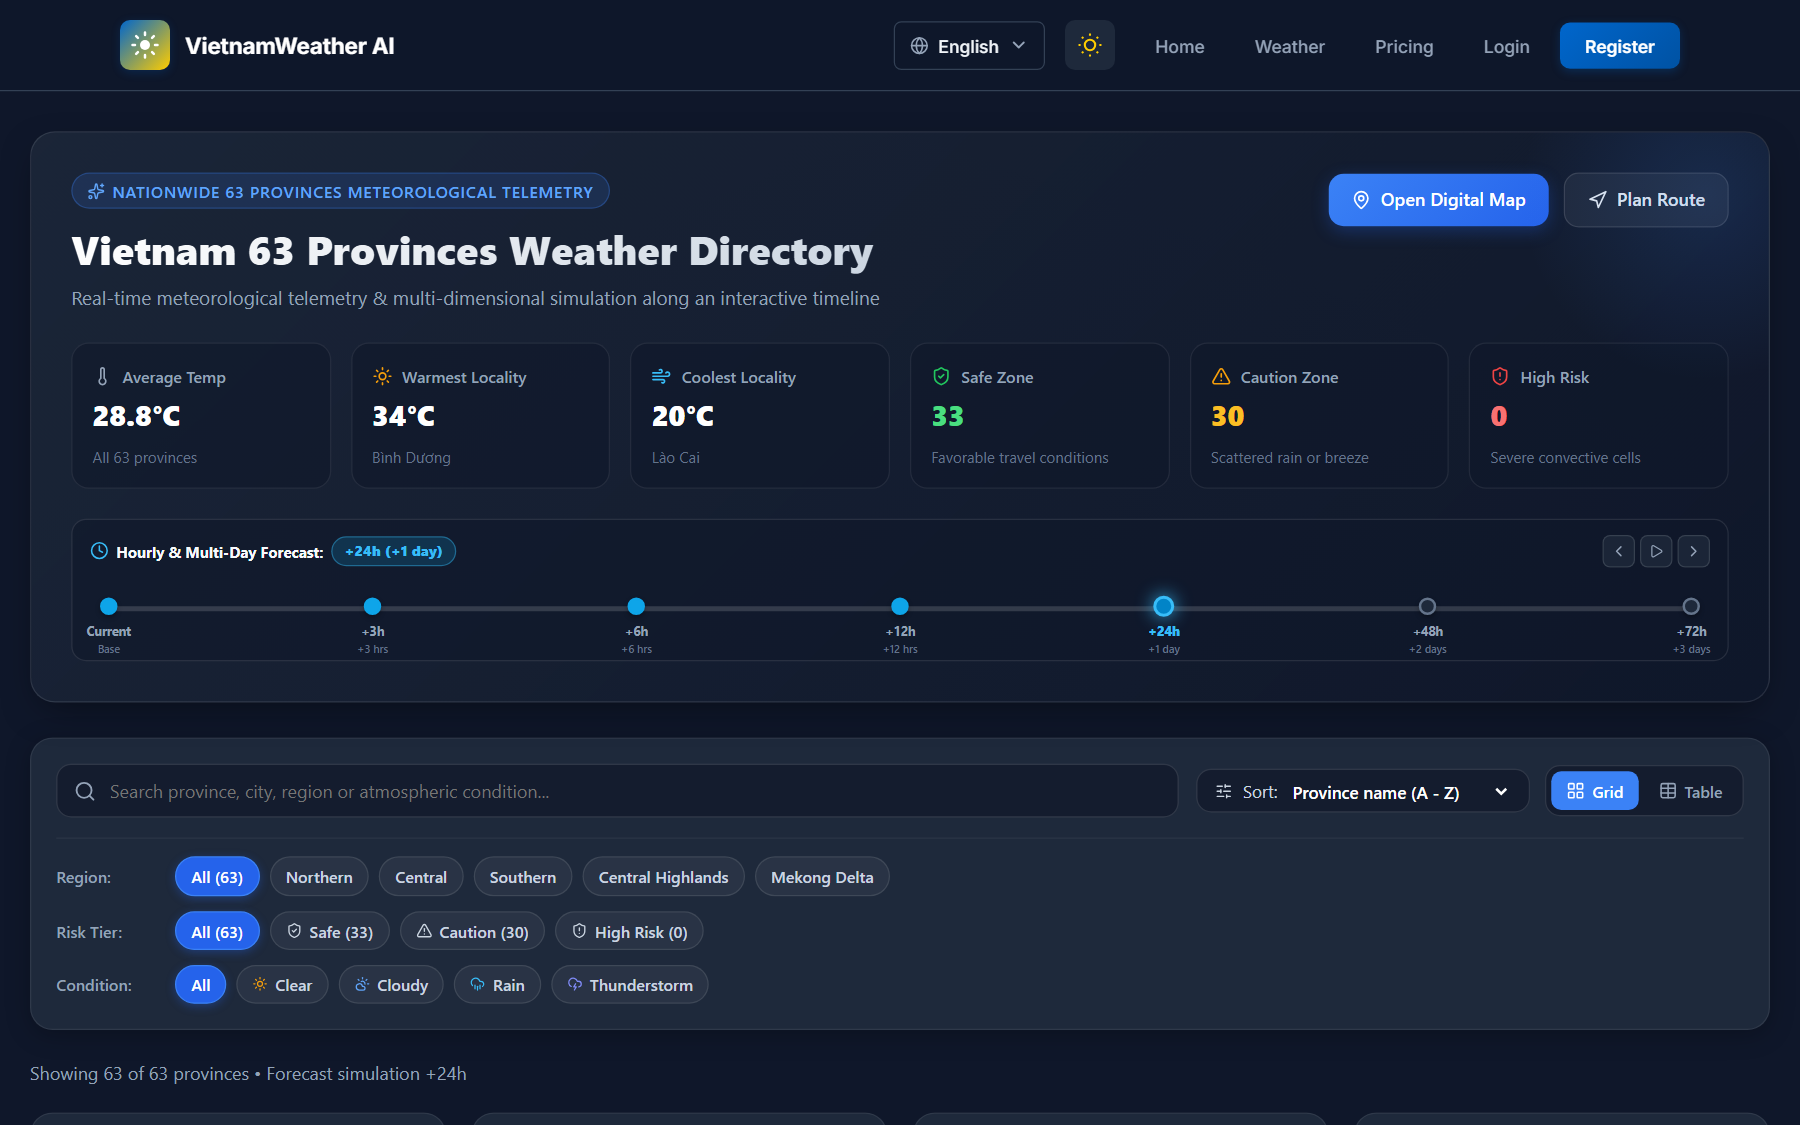
\includegraphics[width=\textwidth]{figures/ui_weather_timeline_24h.png}
    \caption{Mô phỏng dự báo khi kéo tới mốc +24h (1 ngày sau)}
    \label{fig:ui_weather_timeline_24h_vi}
\end{subfigure}
\hfill
\begin{subfigure}[b]{0.48\textwidth}
    \centering
    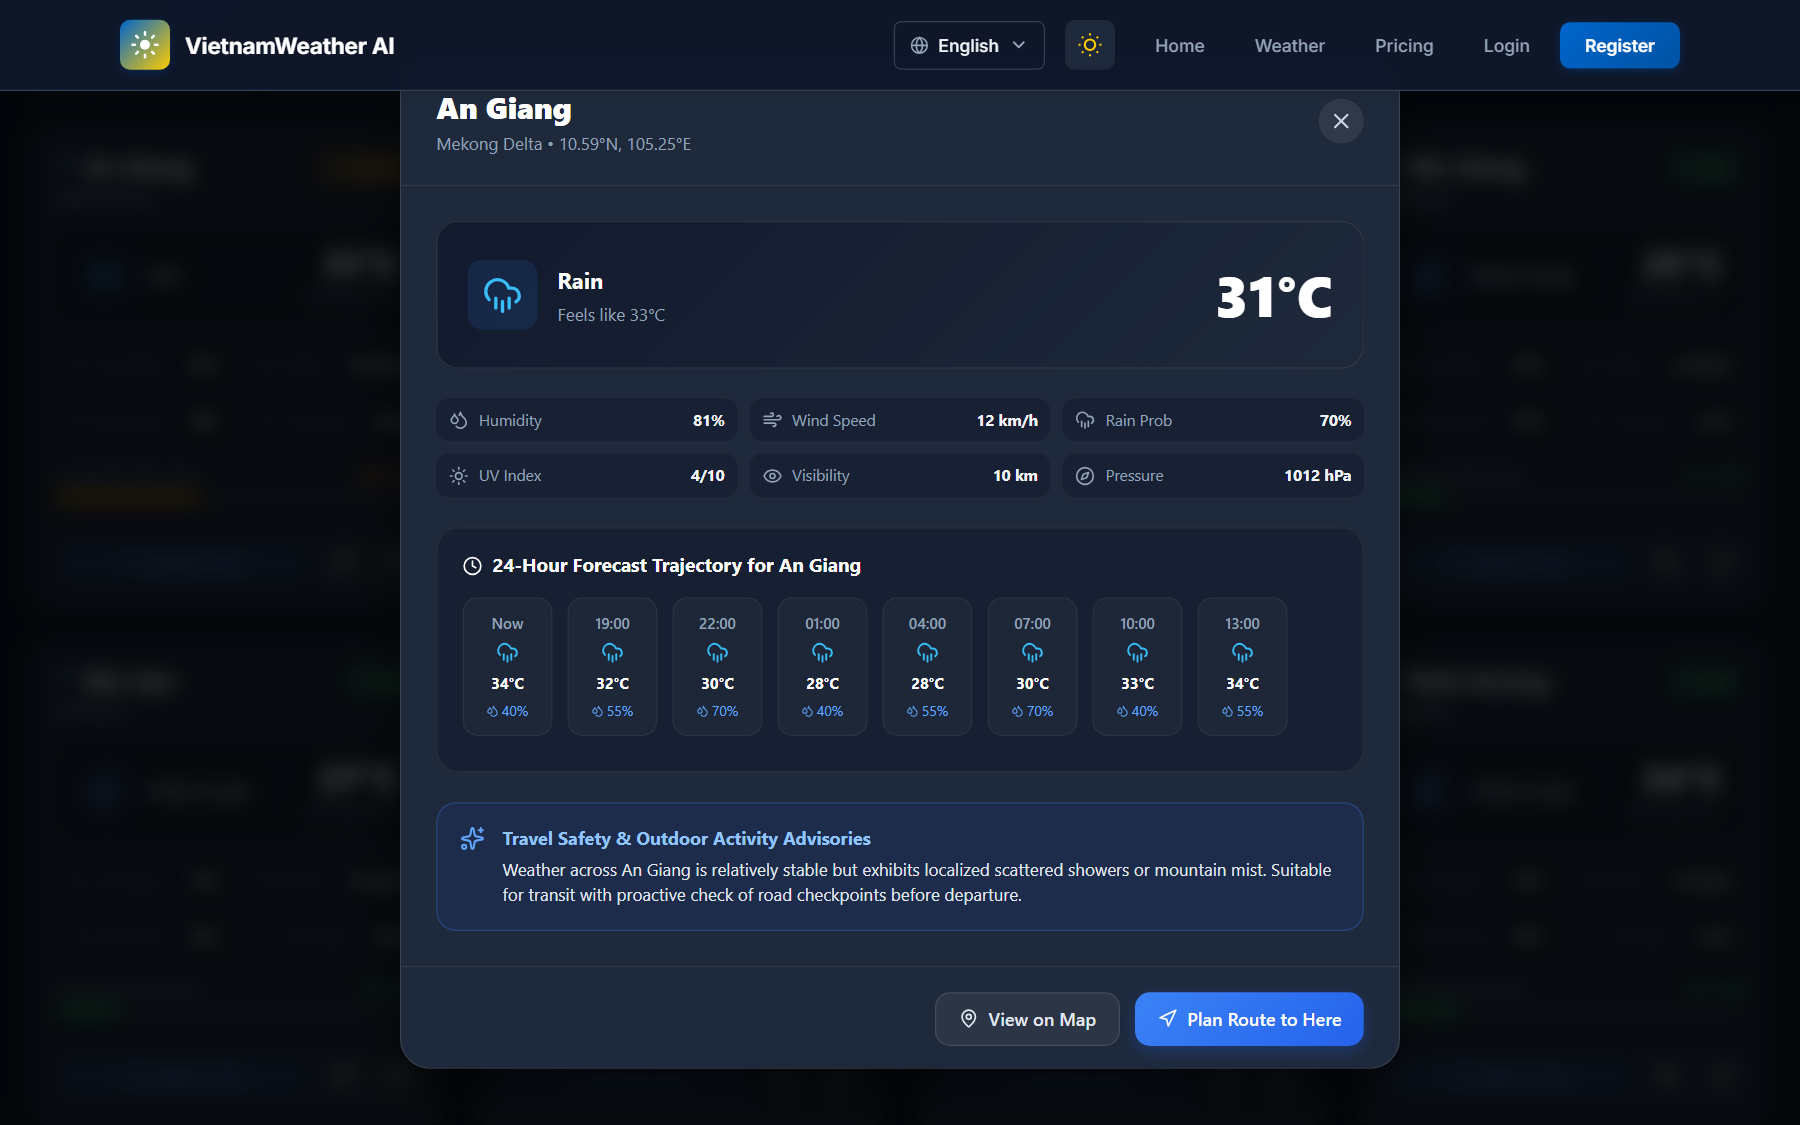
\includegraphics[width=\textwidth]{figures/ui_weather_modal.png}
    \caption{Cửa sổ chi tiết xu hướng 24h \& Khuyến nghị an toàn AI}
    \label{fig:ui_weather_modal_vi}
\end{subfigure}
\caption[Giao diện Mô phỏng Dòng thời gian và Cửa sổ Chi tiết Cấp tỉnh]{Phân hệ giao diện Thời tiết chuyên sâu: (a) Toàn bộ 63 tỉnh thành tự động cập nhật nhiệt độ và mức độ rủi ro khi rê kéo thanh trượt thời gian tới mốc +24h; (b) Cửa sổ phân tích chi tiết cấp tỉnh với xu hướng thời tiết 24 giờ và khuyến cáo an toàn di chuyển thông minh.}
\label{fig:ui_weather_detail_features_vi}
\end{figure}

\begin{figure}[htbp]
\centering
\begin{subfigure}[b]{0.48\textwidth}
    \centering
    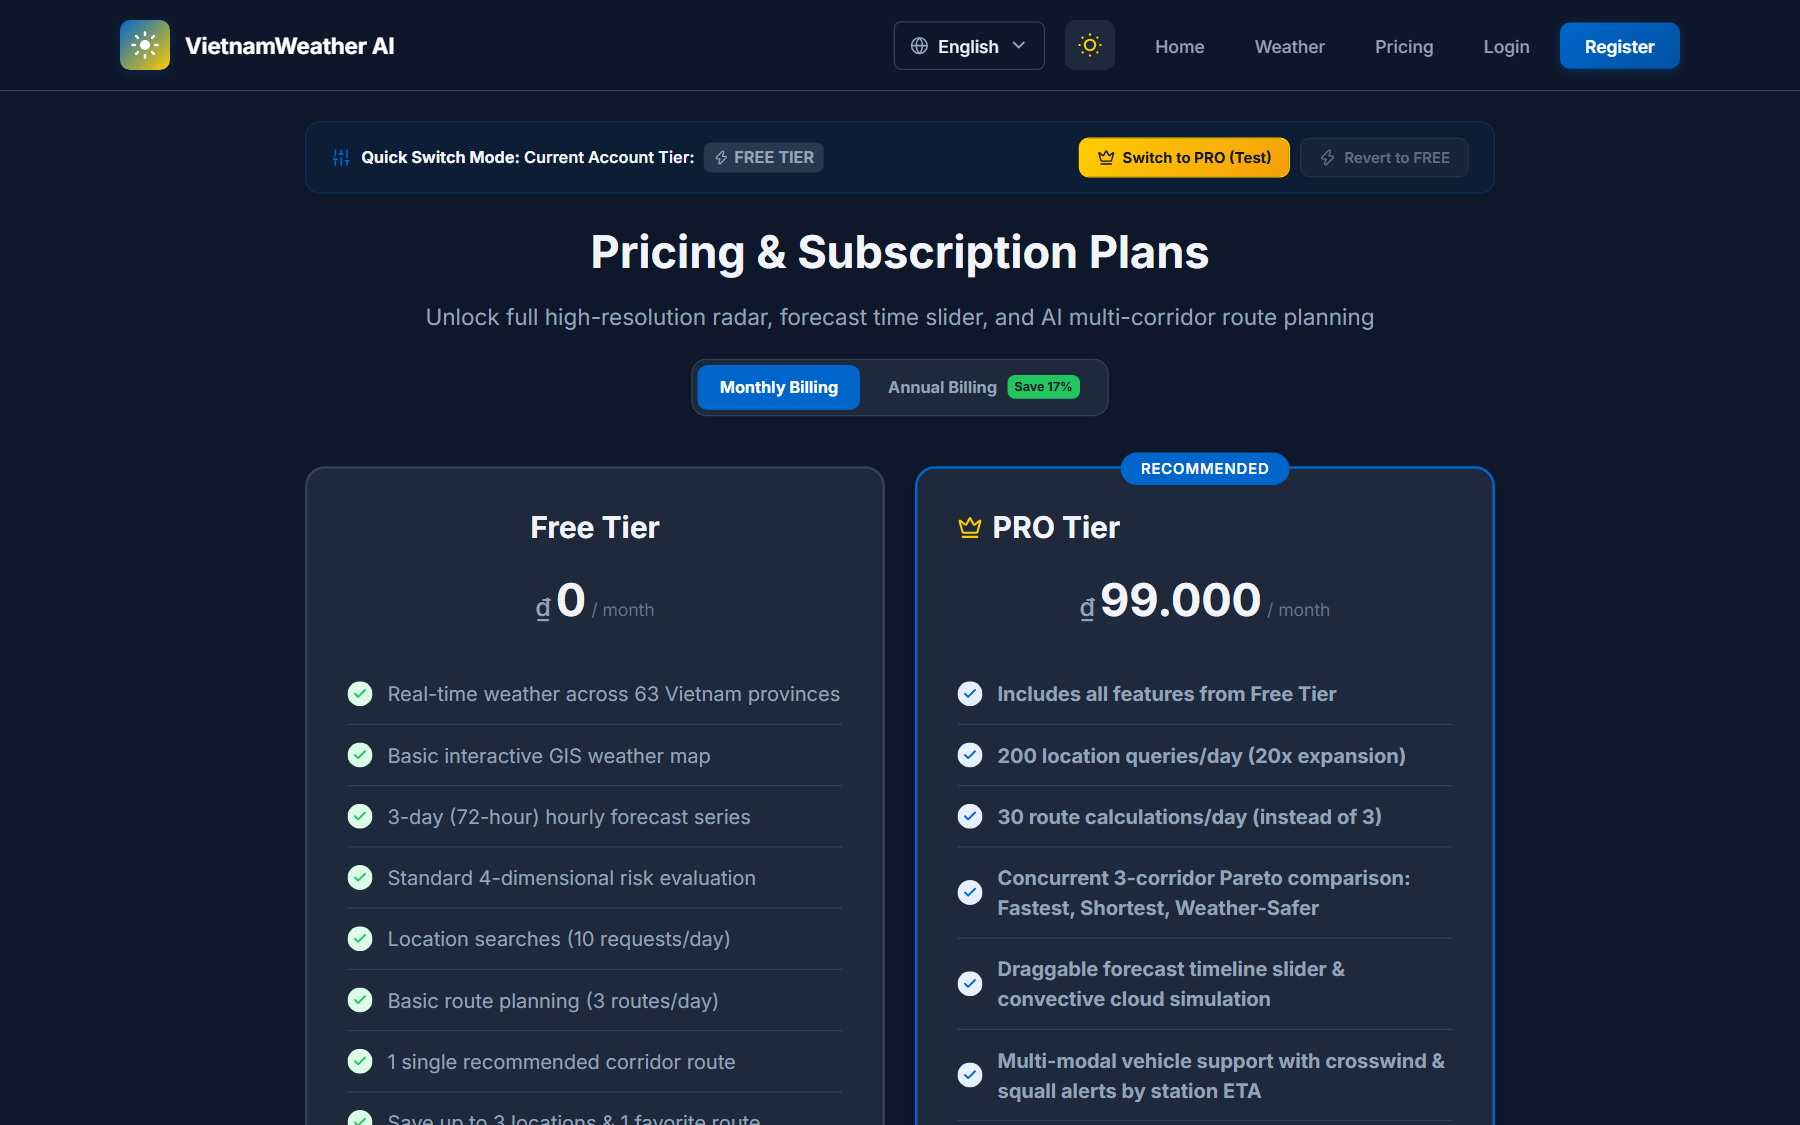
\includegraphics[width=\textwidth]{figures/ui_pricing.png}
    \caption{Bảng giá và Đối sánh quyền lợi Free -- PRO}
    \label{fig:ui_pricing_vi}
\end{subfigure}
\hfill
\begin{subfigure}[b]{0.48\textwidth}
    \centering
    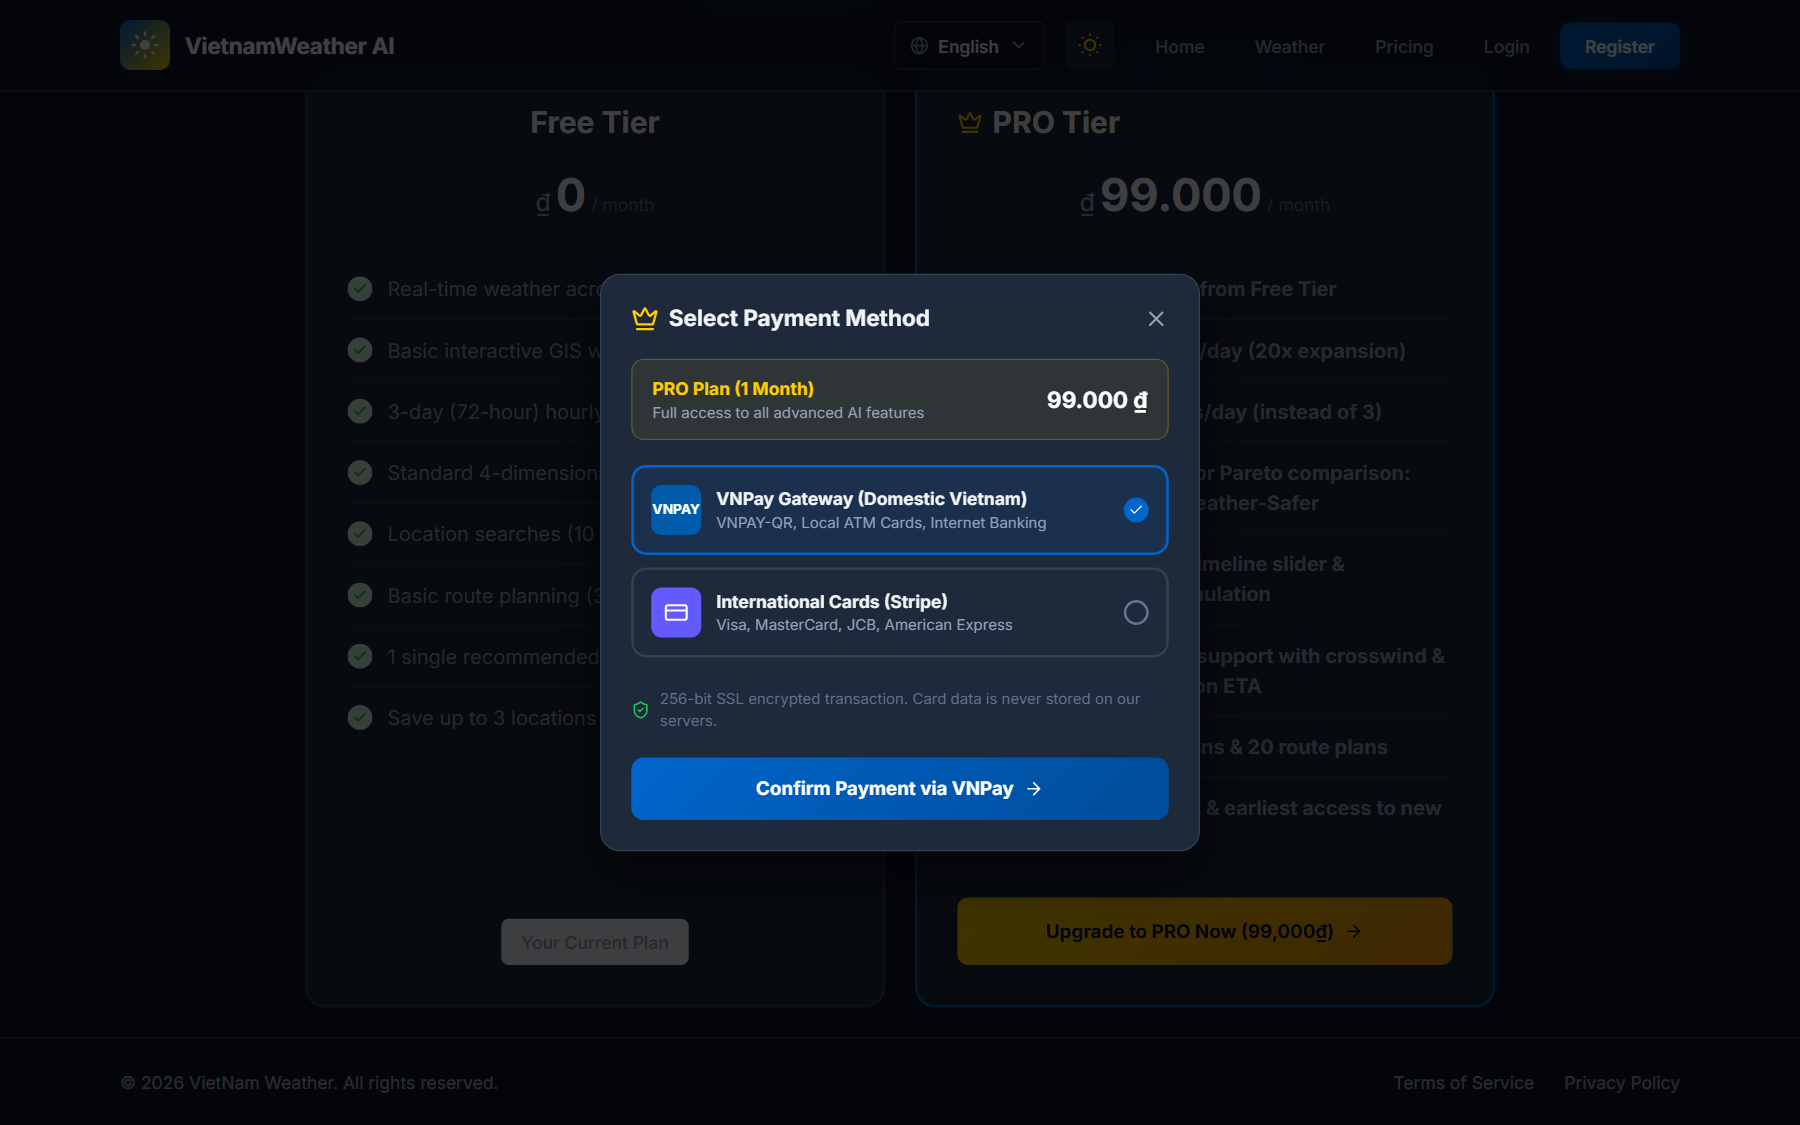
\includegraphics[width=\textwidth]{figures/ui_checkout.png}
    \caption{Cửa sổ thanh toán đa cổng (VNPay \& Stripe)}
    \label{fig:ui_checkout_vi}
\end{subfigure}
\caption[Phân hệ Bảng giá dịch vụ và Cổng thanh toán trực tuyến]{Phân hệ Bảng giá dịch vụ và Cổng thanh toán trực tuyến của nền tảng VietForecast: (a) Giao diện đối sánh quyền lợi hai gói cước Free và PRO với nút chuyển đổi chu kỳ tháng/năm; (b) Cửa sổ thanh toán tích hợp cổng nội địa VNPay (VNPAY-QR, thẻ ATM) và cổng quốc tế Stripe (Visa, MasterCard) bảo mật chuẩn SSL 256-bit.}
\label{fig:ui_monetization_vi}
\end{figure}

\section{Tóm tắt chương}
\label{sec:evaluation_summary}

Chương~\ref{ch:evaluation} đã trình bày hệ thống kết quả đánh giá thực nghiệm toàn diện trên nền tảng VietForecast với các kết quả định lượng nổi bật:
\begin{itemize}
    \item[-] \textit{Về mặt an toàn định tuyến}: Thuật toán Weather-Safer chứng minh khả năng loại bỏ tới $87,2\%$ các điểm rủi ro thời tiết cực đoan trên cả ba hành lang trọng điểm, trong khi mức tăng thời gian di chuyển trung bình được kiểm soát nghiêm ngặt dưới $8,9\%$ và mức tăng cự ly dưới $4,7\%$. Cơ chế phân hóa theo phương tiện đã cảnh báo chính xác nguy cơ gió tạt nguy hiểm đối với người đi xe máy.
    \item[-] \textit{Về mặt hiệu năng hệ thống}: Cây chỉ mục không gian PostGIS GiST hai giai đoạn giúp giảm độ trễ truy vấn hành lang xuống chỉ còn $11,4$~ms trên 100.000 điểm trạm (nhanh hơn 36,9 lần so với quét tuần tự). Máy chủ Fastify API đạt thông lượng trên 2.485~req/s với độ trễ $p_{95} = 12,8$~ms và tỷ lệ lỗi 0,0\%. Cơ chế Circuit Breaker ngắt mạch an toàn trong 60 giây khi có sự cố từ nhà cung cấp ngoài.
    \item[-] \textit{Về mặt trí tuệ nhân tạo}: Trợ lý AI đạt độ chính xác gọi hàm $96,2\%$, tỷ lệ bảo chứng trích dẫn thực nghiệm $97,2\%$, kiểm soát và giảm thiểu tỷ lệ ảo giác thông tin xuống còn $1,8\%$ (giảm hơn $94\%$ so với mô hình không ràng buộc) và chuyển đổi mượt mà sang bộ dự phòng tất định với độ trễ $2,2$~ms khi mất kết nối mạng.
    \item[-] \textit{Về mặt trải nghiệm người dùng}: Giao diện WebGL tương tác đạt điểm số SUS xuất sắc $84,6/100$ điểm (Hạng A), chứng minh tính khả dụng, độ tin cậy và sự đón nhận tích cực từ cộng đồng người dùng thực tế.
\end{itemize}

Các kết quả thực nghiệm vững chắc này khẳng định toàn bộ các mục tiêu nghiên cứu và phát triển đặt ra ban đầu đã được hiện thực hóa trọn vẹn, đặt nền tảng khoa học cho phần tổng kết và các đề xuất phát triển trong tương lai tại Chương~\ref{ch:conclusion}.
